\documentclass[3p]{elsarticle}
\usepackage{amsmath}
\usepackage{amssymb}
\usepackage{natbib}
\usepackage{graphicx}
\usepackage{subfigure}
\usepackage{hyperref}
\usepackage{setspace}
\usepackage{listings}
\usepackage[utf8]{inputenc}
\hyphenation{}

\journal{PS651/PS688} 

\begin{document}
\begin{frontmatter}

\title{The Race to the Bund: Aggregate European and State-Level Integration from the EEC to Present}

\author{Michael J. Bommarito II}
\address{Department of Political Science, University of Michigan, Ann Arbor}
\address{Department of Financial Engineering, University of Michigan, Ann Arbor}
\address{Center for the Study of Complex Systems, University of Michigan, Ann Arbor}
\date{\today}

\singlespacing

\begin{abstract}
Many scholars point to the decreasing yield spread between the benchmark German bund and other European states as a sign of unprecedented European integration since Maastricht.  There are two possible issues with this claim.  First, without a historical perspective on sovereign bond yields and their comovements, researchers cannot determine how current levels of integration compare to previous periods of European history.  To my knowledge, no previous research examines European yields from the formation of the ECSC or EEC to present, let alone pre-war spreads.  Second, the first two moments of yield spreads do not necessarily capture meaningful integration.  While the spreads are certainly an important measure, we can better assess integration by examining the correlation of these yields.  In this article, I address both of these issues as follows.  First, I describe an alternative method of measuring integration in the sovereign bond market based on an eigendecomposition of the time-dependent correlation of yields and their first-order differences.  This approach better measures integration than standard methods because it takes into account the degree to which a single dimension explains the structure and movement of yields.  Second, I construct a dataset of ten-year sovereign bond yields for the EU-15 countries from 1987 to 2010, as well as subsets of these 15 countries from 1958-2010 and from 1872-1913.  I then apply both standard yield spread analysis and the method proposed in this article to these three samples.  The results of the standard yield spread analysis indicate that Europe has seen previous periods of comparable financial integration.  However, based on the alternative method of this article, integration did not occur until the Single European Act of 1987 and the Maastricht Treaty of 1993.  A period of stable and high integration is observed following the adoption of the Euro in 1999.  Furthermore, both methods show that the recent global real estate and European fiscal crises have significantly degraded financial integration to a level not seen since Maastricht.  In summary, this article contributes both a novel and useful methodological approach and a historical basis on which to evaluate modern European integration in the sovereign bond market.
\end{abstract}

\begin{keyword}
Europe \sep European Union \sep integration \sep sovereign bonds \sep yield spread \sep yield correlation
\end{keyword}
\end{frontmatter}

\doublespacing

\section{Introduction}
Throughout its post-war history, Europe has seen the creation and expansion of supranational organizations aimed at economic integration.  From the formation of the EEC in the 1957 Treaty of Rome to the European Union in the 1992 Maastricht Treaty, European states have exchanged autonomy over certain economic and political institutions for the pursuit of economic growth and stability.  While each reform or expansion was designed to increase the degree of economic integration, the short-term and long-term success of these agreements in promoting integration is often debated.

By many measures, Europe is clearly more integrated than at any point in recent history (\cite{Molle1980}, \cite{Molle1988}, \cite{EC2006}).  Measures of per-capita wealth have converged significantly relative to early post-war levels.  As of 2004, intra-EU trade has risen to approximately two-thirds of total trade and one-third of total EU GDP.  Recent research highlights, however, a decrease in the rate of convergence, and, in some cases, even the possibility of divergence (\cite{Fagerberg1996}, \cite{Cappelen1999}, \cite{PenaCasas2009}).  Furthermore, there is debate in the literature as to what factors actually drive convergence at the state level (\cite{Brada2001}, \cite{Cappelen2003}, \cite{Gray2009}).  It seems na\"ive to assume that EU membership alone, in absence of sound economic fundamentals or reform, is responsible for the improvement seen in many European countries.

According to \cite{Gray2009}, three theories might explain what factors drive state-level convergence.  The first theory argues that EU membership and constraints are unrelated to improved economic variables, as states would not join organizations whose rules they did not already comply with (\cite{Downs1996}, \cite{VonStein2005}).  The second theory instead suggests that the process of accession, in which states often undertake significant reform to comply with the \textit{acquis communautaire},  explains the improvement in the state's economic and political institutions; that negotiations and eventual acceptance cooccur is merely a coincedence (\cite{Schimmelfennig2005}, \cite{Vachudova2001}).  The third theory is based on signalling and argues that the EU's signal of acceptance decreases the risk of asymmetric information for private investors.  Arbitrating between and exploring alternatives to these theories improves our understanding of what factors drive improvement in real human outcomes.  This article contributes an additional perspective to the question by examining both aggregate European and state-level integration through the sovereign bond market.  

Research in political science and finance on integration using sovereign bonds can be divided into two groups - one that focuses on integration as measured by standard econometric models, and one that focuses on the ratings of sovereign bonds in the context of political, legal, and economic institutions.  The econometric study of bond market integration is a recent phenomenon.  In fact, the first modern results on correlation between international bond markets were only published by Levy and Lerman in 1988 (\cite{Levy1988}) and Burik and Ennis in 1990 (\cite{Burik1990}).  These studies are standard explorations in modern portfolio theory, driven by Markowitz's framework for portfolio selection and optimization (\cite{Markowitz1959}).  This framework takes as input a set of assets, along with estimates of their expected return and standard deviation, and produces a vector of portfolio weights.\footnote{In order to produce this vector of portfolio weights, portfolio selection is framed as a quadratic programming optimization problem.  The goal is to minimize the risk of a portfolio for every level of return; that is, let an investor choose their desired level of return, and solve for the resulting minimum-risk portfolio.  The solution to this problem, the set of all efficient combinations of risk and return, is known as the ``efficient fronter'' - points outside the frontier are not attainable given the market's assets, points on the frontier are attainable and efficient for a given level of return, and points inside the frontier are attainable but inefficient.  This frontier is often described as ``bullet-shaped.''}  These weights indicate the proportion of a portfolio that is held in each asset.  Using this framework, they show that optimal portfolios include international sovereign and corporate bonds, confirming that there are previously unobserved diversification benefits in these markets.  This ``diversification'' represents a decrease in correlation of business cycle and risk factors, and therefore corresponds to market segmentation or less integration.  This finding and increased data availability have sparked further research into international bond markets.

Clare, Maras, and Thomas (\cite{Clare1995}) are the first to study the integration of international bond markets per se.  In their 1995 article \textit{The integration and efficiency of international bond markets}, they apply both Engle-Granger and Dickey-Fuller tests of cointegration  and find a relatively low correlation between the total return of international bond markets during the 1980s.  Despite their interesting findings, however, they provide little discussion or explanation of the difference between bond and equity market integration.   Solnik et al. (\cite{Solnik1996}) and Christiansen and Pigott (\cite{Christiansen1997}) further examine this correlation over longer periods of time.  They find that the links between international bond markets strengthened between the 1960s and 1980s but that there has been no directional trend since then.  Again, however, there is little theory or explanation behind these observations. Clare later addresses this issue with Lekkos in his 2000 article \textit{An analysis of the relationship between international bond markets}, in which they regress out systemic and factor-specific risk components.  After compensating for this alternative model, they find that integration has increased in the prior decade.  Since these articles, sovereign bonds have often been used to assess integration.  Groups such as the Federal Reserve, ECB, and the IMF have directly applied yield spreads as measurements of integration, either in the case of EU member states with each other or emerging economies with developed economies (\cite{ECB2004}, \cite{ECB2005}, \cite{ECB2007}, \cite{FRBSF2008}, \cite{FRBSF2004}, \cite{Ekinci2007}).

The second category in this literature on sovereign bonds focuses on the determinants of and changes in credit ratings.  These ratings, produced by credit rating agencies such as Moodys, S\&P, and Fitch, convey the expert-assessed risk of failure to service debt.  Unlike yields, however, they are determined by single agencies and only represent ordinal risk categories.  Furthermore, their accuracy and credibility have recently come under attack by researchers and policy advocates in numerous markets (\cite{Hunt2009}, \cite{Frost2006}, \cite{Kuhner2001}).  Notable examples of articles that examine these ratings, especially in the context of emerging markets, include \cite{Cantor1996}, \cite{Durbin1999}, \cite{Biglaiser2007}.  

This article falls into the former of the two categories.  While the methods herein are not traditionally econometric, the methods are based on estimating parameters of a model for sovereign bond yields.  By observing changes in these parameters, possible changes in the real world can be identified.  Using these yields, The remainder of this article is organized as follows: in section \ref{sec:data}, I describe the dataset compiled to study the EU-15 between 1987 and 2010 and two subsets of this group from 1872-1913 and 1958-2010; in section \ref{sec:methods}, I provide an explanation of the two methods used to assess integration: yield spread and yield comovement; in section \ref{sec:results}, I apply these two methods and present the results for both the EU-12 and EU-15 datasets.  Finally, in section \ref{sec:discussion}, I provide a summary discussion of these results and conclude.

\section{Data}
\label{sec:data}
The focus of this article is on the sovereign bond markets of the EU-15 states: Austria, Belgium, Germany, Denmark, Spain, Finland, France, the United Kingdom, Greece, Ireland, Italy, Luxembourg, Netherlands, Portugal, and Sweden.  I have obtained the entire history of ten-year sovereign bond yields for each of these countries from Global Financial Data (\cite{GFD2010}).  For a variety of reasons, a number of these countries did not have outstanding issues at the ten-year maturity during the period prior to World War I or after World War II.  Yields on all 15 member countries at this maturity are only available from January 1987 forward.\footnote{The recent fiscal crises in the Eurozone have actually led countries such as Greece to significantly reduce their issuance on the public markets.  If countries were to completely exit the public market for this debt and rely entirely on ECB or IMF mechanisms for funding, then this measurement strategy clearly cannot work.}

In order to examine the EU-15 countries over a long period of time pre-Maastricht, I have selected two periods of time in which a substantial number of these countries had outstanding ten-year issues that traded.  The first of these samples is obtained by removing Finland, Greece, and Luxembourg from the post-1945 data.  I will refer to the remaining twelve countries as the EU-12 throughout the remainder of the article.\footnote{The European Union has recently begun to refer to a number of the recently admitted states as EU 10 and EU 12.  The EU-12 discussed in this paper have no relation to these recent and rapidly changing EU conventions.}  The remaining time period in which all bonds traded is from January 31st, 1958 to November 5th, 2010, and the remaining twelve countries are Austria, Belgium, Germany, Denmark, Spain, France, the United Kingdom, Ireland, Italy, the Netherlands, Portugal, and Sweden.  During the period from 1958 to 1970, these ten-year yields are available at monthly frequency on the last day of each month.  Figure \ref{fig:data_eu12} in Appendix A shows the number of observations available for all countries in each year of the dataset. Beginning in 1970, this frequency increases to between 15 and 18 releases per year, and in April of 1978, bond markets began trading these assets each business day and yields are thereafter available at daily frequency.

The second pre-Maastricht sample is selected to gain insight into European sovereign bond markets before the World Wars.  By removing Austria, Finland, the United Kingdom, Greece, Ireland, and Luxembourg, a dataset is obtained that spans from the original unification of Germany in 1872 to the end of 1913.  I refer to this sample as the EU-9 sample, as there are nine members of the EU-15 group included.  For the first six years of this sample, data is available at monthly frequency.  Beginning in 1880, however, the data is reported at slightly higher than weekly frequency.  Figure \ref{fig:data_eu9} in Appendix A shows the number of observations available for all countries in each year of the dataset.

The third sample includes all EU-15 member states at daily frequency from February 1987 to April 2010, and I refer to this as the EU-15 sample.  Due to the fiscal crisis in the Eurozone in the spring of 2010, Greek bonds did not trade for an extended period and the dataset therefore does not extend as far as the EU-12 sample from 1958-2010.

\section{Methods}
\label{sec:methods}
\subsection{Yield Spread}
Researchers have used bond yields to assess economic integration for many years and in many contexts.  The most common method of assessing integration is to compare the yield of a group of countries to a benchmark yield.  This yield might be the yield of another country's sovereign bonds, such as the United States or Germany, or a private borrowing rate such as the Federal Funds rate, the London InterBank Offered Rate (LIBOR), or the Euro InterBank Offered Rate (EURIBOR).\footnote{The most well-known spread is the ``TED'' spread, which measures the difference between the three-month yields of U.S. Treasury bills and three-month LIBOR.  In this context, the spread measures the perceived credit risk of the economy, based on the assumption that short-term U.S. Treasury solvency is guaranteed.}  The European Central Bank uses this method to assess Eurozone integration in its regular publication, \textit{Financial integration in the Euro area} (\cite{ECB2004}, \cite{ECB2005}, \cite{ECB2007}).  In its 2004 publication, the ECB explains the intuition behind this method as follows:
\begin{quote}
	... the strongest measures of financial integration are those based on the law of one price.  Insofar as government bonds are sufficiently homogeneous across the various euro area markets, one can directly test the law of one price by comparing the yields on local government bonds across countries. If we assume that the degree of systematic risk is identical across countries, then risk premia should also be identical in perfectly integrated markets, and hence yields on government bonds with the same maturity should be identical as well.
\end{quote}

This analysis can be formalized by considering a benchmark yield $y_b(t)$ and a set of N comparison yields $y_i(t), i = 1, \cdots, N$.  It is important that the bonds from which these $y$'s are calculated are as homogeneous as possible; ideally, the bonds will all be on-the-run with the same maturity, liquidity, coupon schedule, issuance date, and embedded options.  Though this is almost never possible in practice, it is easier to accomplish with some maturities than others.  For instance, the ten-year bond markets are much more active than other maturities, and therefore it is easier to find comparable bond issuances.

Based on this benchmark yield $y_b(t)$ and the comparision yields $y_i(t)$, we can calculate the spread on yield $i$ relative to $b$ simply by subtraction - $\hat{y}_i(t) = y_i(t) - y_b(t)$.  There are two points to note for this spread $\hat{y}_i(t)$.  First, the spread is a function of time $t$ and will change according to the market's perception of risk and integration.  Second, the spread is not necessarily strictly positive; in some conditions or time periods, the chosen benchmark may not represent the least risky asset.  However, if a chosen benchmark results in spreads that are rarely positive, then it is likely an inappropriate choice.

In situations such as EU integration studies, there are many comparision yields.  For example, in the EU-9, EU-12, and EU-15 samples described, there are 8, 11, and 14 comparison yields respectively.  To summarize the collective behavior of these individual yields, researchers often use the first two moments of the distribution of spreads at a fixed time, not across time for a single state.  The mean $\mu_y(t)$ and standard deviation $\sigma_y(t)$ of spread are given by:
\begin{align*}
	\mu_y(t) =& \frac{1}{N} \sum_{i=1}^N \hat{y}_i(t)\\
	\sigma_y(t) =& \sqrt{\frac{1}{N-1} \sum_{i=1}^N (\hat{y}_i(t) - \mu_y(t))^2}
\end{align*}
Though each yield spread often has its own interesting spike or story, I will rely primarily on this mean and standard deviation of spread to characterize overall integration.  To summarize, we can infer increased integration by noting either (1) decreasing absolute value of mean spread and (2) decreasing standard deviation of spreads.

Using this logic and ten-year yields with a German benchmark, the ECB shows that both the spread and the dispersion of spread has decreased over the period from 1993 to 2007 for EU member states.  In their 2004 publication, they show that, with the exception of Greece, spreads have decreased to below 30 basis points by 1998.\footnote{Though the 2005 and 2007 publications also consider this spread, they do not provide as many figures or tables on government bond market integration.}  Dispersion had fallen from 5\% at the outset of Maastricht to 1\% by 1999, remaining steady near zero from 2001 onwards.  These results indicate that sovereign bond markets was very well integrated at the time these reports were published.

However, neither this publication nor any other ECB publication compares the value or trend of yield spreads to periods prior to Maastricht.  Therefore, one way in which this paper contributes to the discussion is by simply repeating these tests on spread and spread dispersion in periods prior to the Maastricht Treaty.

\subsection{Yield Correlation}
In the above section, I summarize the common approach to measuring integration through yield spread.  One important factor that affects these spreads, however, is the type of global monetary system.  In the presence of a gold standard, exchange rate risk is removed from the pricing of sovereign bonds.  In this case, the difference in yields across countries will likely be smaller in absolute value than in a fiat system, as a term that is stochastic in fiat systems is fixed.  Since many studies examine periods that span both gold and fiat systems, spread analyses are confounded by switches between monetary systems such as the end of Bretton Woods in 1971.  In order to address this issue, I deviate significantly from prior research by proposing a method of decomposing the correlation of yield and its first-order differences.  This analysis is based on recent techniques in correlation developed in statistical mechanics and empirical finance, and is less prone to this monetary system criticism than spread analyses.  

The study of correlation has been fundamental to the mathematics of finance since Markowitz first introduced his theory of portfolio selection (\cite{Markowitz1952}).  Since then, time-dependent correlation has been used to study the dynamics of assets both within and across markets and on time scales ranging from minutes to years (\cite{Drozdz2001}, \cite{Heimo2007}).  In the recent past, methods developed in applied spectral analysis and Random Matrix Theory (RMT) have received significant attention in the study of correlation in financial markets.  Many of these studies have focused on evaluating theoretical predictions (\cite{Laloux1998}, \cite{Laloux2000}, \cite{Conlon2009}) and uncovering interesting substructures and behaviors in markets.  

One method of analysis in these studies is to observe the time series of the maximum eigenvalue of the time-dependent correlation matrix.  Recent literature has begun to investigate the use of this maximum eigenvalue time series in risk management and trading strategies.  In \textit{A profitable trading and risk management strategy despite transaction cost}, Duran and Bommarito successfully apply the maximum eigenvalue of a time-dependent correlation matrix in a predictive setting for the S\&P 500 (\cite{Duran2010}).  The signal is used as a measure of integration across stocks and prevents the strategy from trading in periods where integration is either abnormally high or low.  The resulting strategy outperforms the market in out-of-sample Monte Carlo simulations with both random subsets of assets on random sub-periods of the dataset.

Based on this success of spectral methods in prediction and identification, it seems reasonable to apply these methods to measure integration in sovereign bond markets as well.  Unlike simple measures of integration such as the yield spread above, spectral characterizations of integration take into account the covariance and dimensionality of the asset relationships.  In the remainder of this section, I will provide a brief explanation of the intuition and process behind this approach.

Models of asset dynamics often consider $N$ uncorrelated assets with a parameterized process governing either their value, such as price, or their first-order differences, such as returns.  The most common choice is to model the process as geometric Brownian motion (GBM), which results in an assumption of normality of asset returns.  This is the model on which much of finance is built, including the Black-Scholes option pricing equation and the Value-at-Risk (VaR) risk management model.  The simplest meaningful extension of this model is to incorporate the covariance $\Sigma$ of these assets into the model.  The components of $\Sigma$ encode linkages, either positive or negative, between these $N$ assets.  In most situations, researchers and practitioners use historical estimates of $\Sigma$ to identify or exploit these linkages.

However, this covariance matrix $\Sigma$ is often assumed to be stationary or constant.  Though this assumption may make sense in certain contexts, it certainly will not hold in situations where technological or political changes directly affect the economy.  Therefore, by assuming that the linkages between assets are inherently time-dependent, researchers can better understand changes in the system they are studying.

The application of this intuition to the sovereign bond market is straightforward.  In this case, bond yields can be modeled as arbitrary processes with time-dependent covariance.  In some periods, market actors may determine that linkages between sovereigns are strong, and, in other periods, weak.  This change in market perception is typically a function of changes in the economic or political institutions or signals issued by governments.  For example, military alliances or bilateral trade agreements produce signals or create institutions that increase dyadic state linkage.  In times of war, allies will likely have positive correlation in their yields, whereas enemies will have negative correlation in their yields.  When one trading partner enters recessionary periods or faces political uncertainty, the economy of the other likely suffers.  In general, the correlation of yields is a good measure of market perception on the relationship between states.

To measure the level of integration, I propose an algorithm based on the eigenvalues of the time-dependent correlation matrix.  This algorithm takes as input an $M x N$ return matrix $R$, where $R_{i,j}$ is the value or difference of the $j^{th}$ asset on the $i^{th}$ period, and $\tau$, the window size for calculating time-dependent correlation.  For each time $t \in (\tau+1, M)$, the windowed estimate of the mean $\hat{\mu}^tau(t)$ and standard deviation $\hat{\sigma}^\tau(t)$ of each asset is calculated.  We can explicitly write this windowed estimate of mean and standard deviation with window size $\tau$ at time $t$ for the $j^{th}$ asset as follows:
\begin{align*}
	\hat{\mu}^\tau_j(t) =& \frac{1}{\tau} \sum_{i = t - \tau + 1}^{t} R_{i,j}\\
	\hat{\sigma}^\tau_j(t) =& \sqrt{\frac{1}{\tau - 1} \sum_{i = t - \tau + 1}^t (R_{i,j} - \hat{\mu}^\tau_j(t))^2}
\end{align*}

These are the standard sample estimates of mean and standard deviation with fixed window often used in practice on asset returns in risk management and trading.  From these first two moments, we can then write the time-dependent empirical correlation matrix $C^\tau(t)$ with window size $\tau$ at time $t$ as
\begin{align*}
	C_{j,k}^\tau(t) =& \frac{\sum_{i = t - \tau + 1}^t (R_{i,j} - \hat{\mu}^\tau_j(t)) (R_{i,k} - \hat{\mu}^\tau_k(t))}{(\tau - 1) \hat{\sigma}^\tau_j(t) \hat{\sigma}^\tau_k(t)}
\end{align*}

Spectral methods then consider the set of eigenvalues $\lambda_i$ and eigenvectors $\nu_i$ that satisfy the following equation
\begin{align*}
	C^\tau(t) \vec{\nu_i} =& \lambda_i \vec{\nu_i}
\end{align*}

For a fixed time, these eigenvalues $\lambda$ and eigenvectors $\nu$ can be interpreted using the same logic as in principal component analysis (PCA).\footnote{Readers are referred to Hardle for further treatment of principal component analysis and related methods (\cite{Hardle2007}).}   Each eigenvalue is proportional to the proportion of variance that its corresponding eigenvector contributes to the system.  In the case of correlation matrices, the sum of the eigenvalues is constrained to be the number of assets of the matrix, and so we can calculate this proportion simply by dividing by $N$.  In the context of markets, the leading eigenvector (the one corresponding to the maximum eigenvalue) is referred to as the ``market'' eigenvector and represents the primary structure of a system.  The higher the proportion of variance explained by the maximum eigenvalue, the more the ``market'' eigenvector is an accurate approximation of the market dynamics.  

Long memories, mean reversion, and significant autocorrelations are frequently observed in empirical yield data (\cite{Baillie1996}, \cite{Mccarthy2004}).  Just as these characteristics may complicate the analysis of yield spreads, they may also affect the estimation of correlation in this context.  One approach to address this issue is to estimate the correlation of the first-order difference of yields.  This can be done simply by replacing the matrix $R$ above with $\Delta R$, where $\Delta$ is the first-order column difference operator.\footnote{Depending on the model of interest rates, these differences may also be transformed by an affine or log function.  In this model, they simply represent the untransformed number of basis points.}  Interpreting the decomposition of this difference correlation matrix is done exactly as described above in the undifferenced case.

We can use the interpretation of this method to assess market integration quickly and simply. A larger maximum eigenvalue implies that the sovereign bond market of the sample is better approximated by a single, integrated market.  Furthermore, the lower the standard deviation of the market eigenvector, the more equally each country contributes to market variance.  Therefore, we can infer increased integration by noting (1) increases in the maximum eigenvalue or (2) decreases in the standard deviation of the leading eigenvector's components.

\section{Results}
\label{sec:results}
In section \ref{sec:methods} above, I have described two methods of assessing the integration of sovereign bond markets.  The first method is based on observations of sovereign bond yield spreads against a benchmark, and we equate increased integration with (1) decreasing absolute value of mean spread and (2) decreasing standard deviation of spread.  The second method is based on a spectral decomposition of the time-dependent correlation matrix of bond yields and their first-order differences.  In this approach, we equate increased integration with (1) increases in the maximum eigenvalue and (2) decreases in the standard deviation of the leading eigenvector's components.

In this section, I apply these two methods to each sample described in section \ref{sec:data} above - the EU-9 sample from 1872-1913, the EU-12 sample from 1958-2010, and the EU-15 sample from 1987-2010.  The EU-9 sample and EU-12 sample are chosen to capture pre-Maastricht Treaty Europe.  The EU-15 sample captures primarily post-Maastricht Europe.  By comparing the results from each of these samples, we can better understand relative levels of sovereign bond market integration.

\subsection{EU-9: 1872-1913}
Figure \ref{fig:de_spread_eu9} displays a summary of the sovereign bond yield spread relative to German bonds for the period from 1872 to 1913.  Panel (a) plots each country's spread over the period.  Notably, Spain's spread spikes following the political instability and revolution surrounding the First Spanish Republic of 1873-1874.  Portuguese spreads also spiked near 1890 in the wake of near-conflict with Britain over North African colonies and the ensuing collapse of the Portuguese government.

Panels (b) and (c) below show the mean and standard deviation of these spreads.  In general, the mean spread relative to the German yield decreases to near zero over the period leading up to World War I.  Between 1900 and 1913, the mean spread never crossed above 50 basis points - a level that the current European sovereign bond market has not crossed below since early 2010.  In general, though marked by brief periods of instability in the Iberian peninsula, the sovereign bond market of the early 20th century is well-integrated by this measure.

\begin{figure}[ht!]
	\centering
	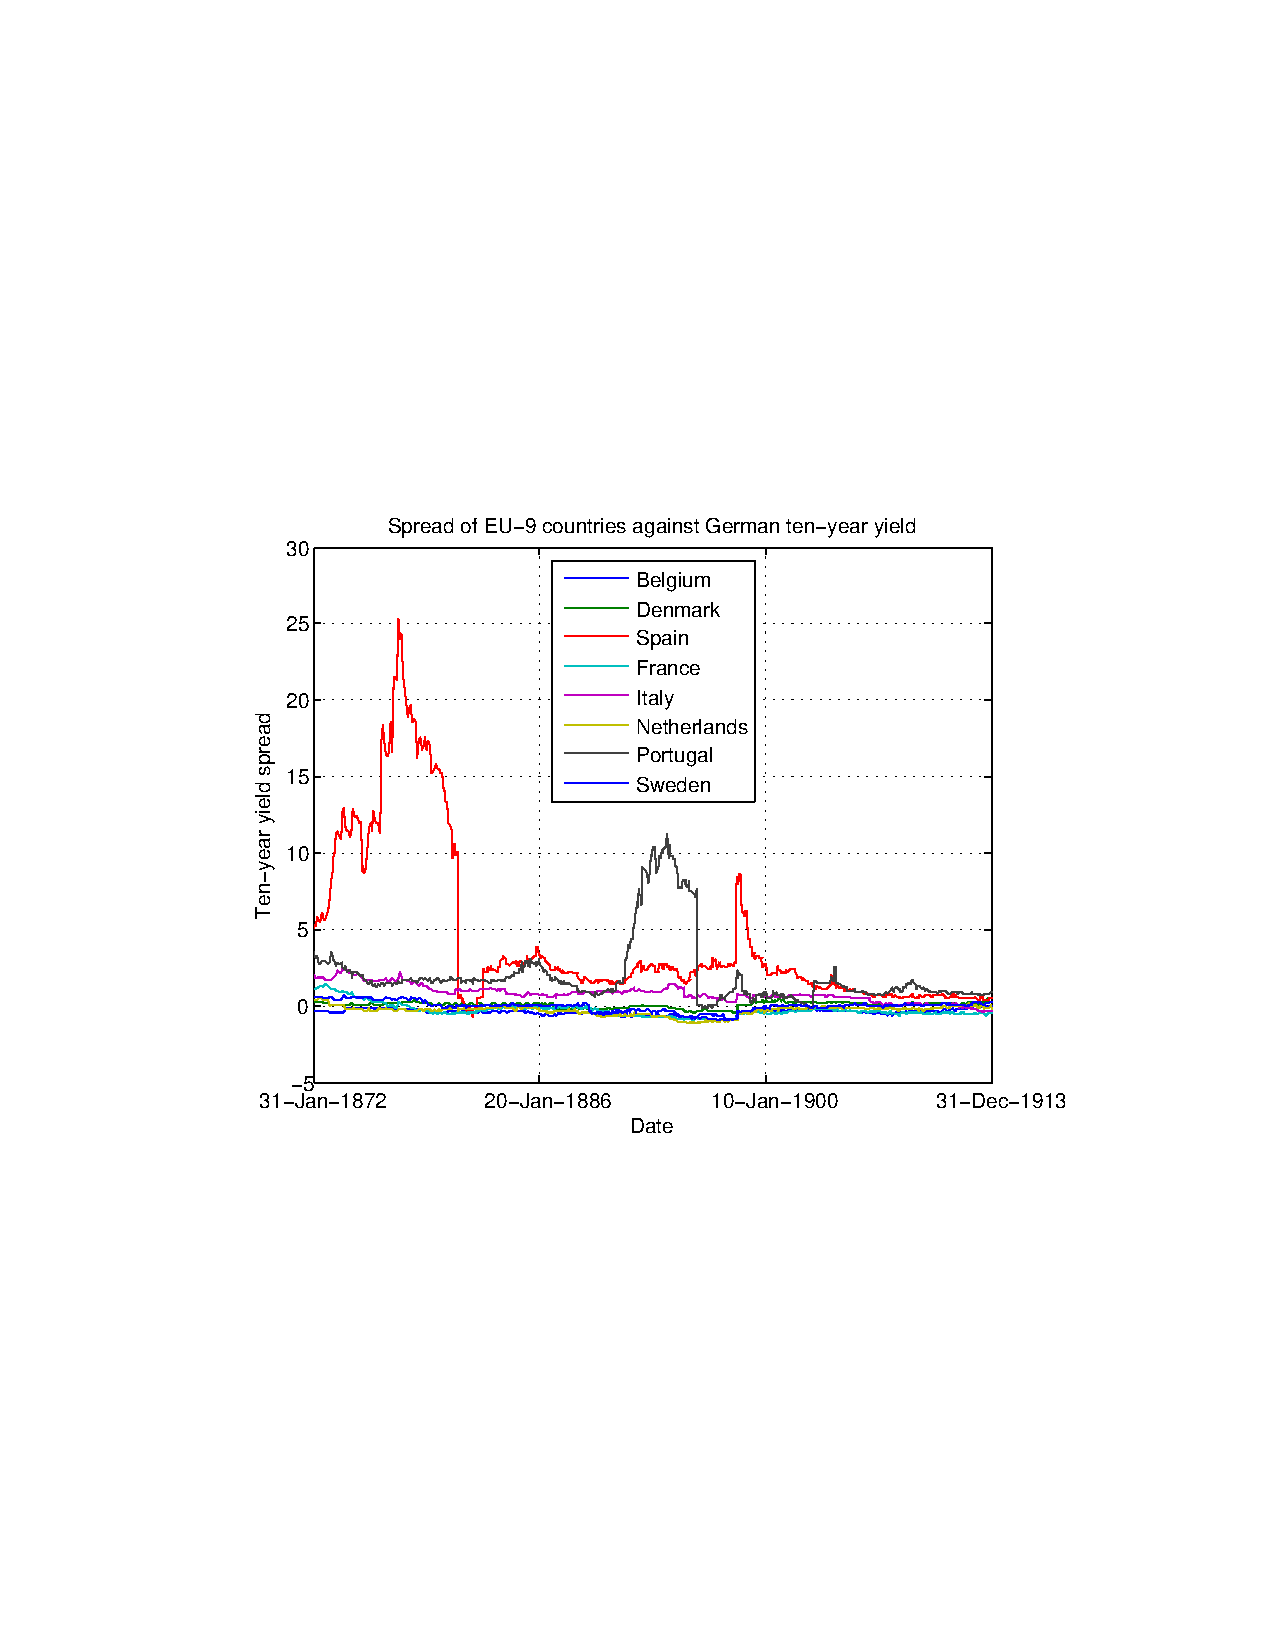
\includegraphics[width=8cm]{fig_de_spread_eu9}\\
	\begin{tabular}{cc}
		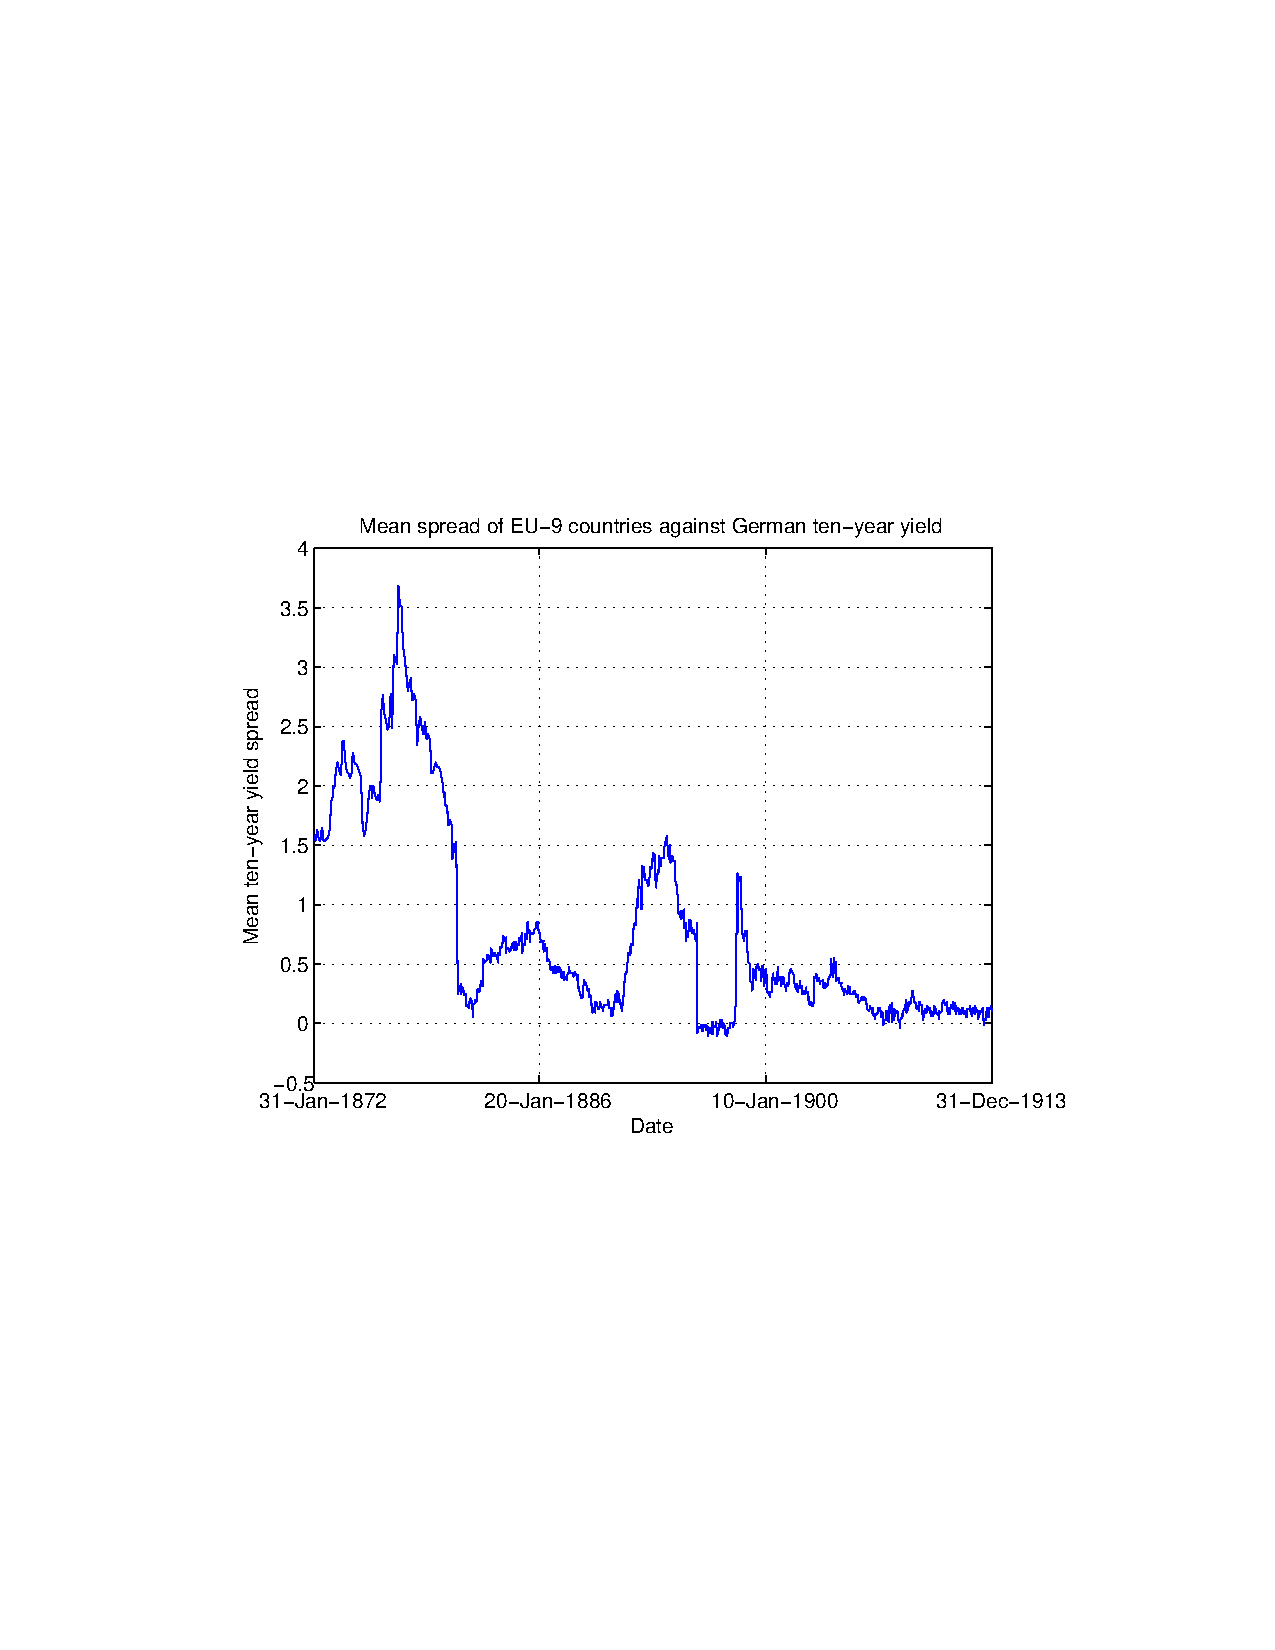
\includegraphics[width=7cm]{fig_de_meanspread_eu9} & 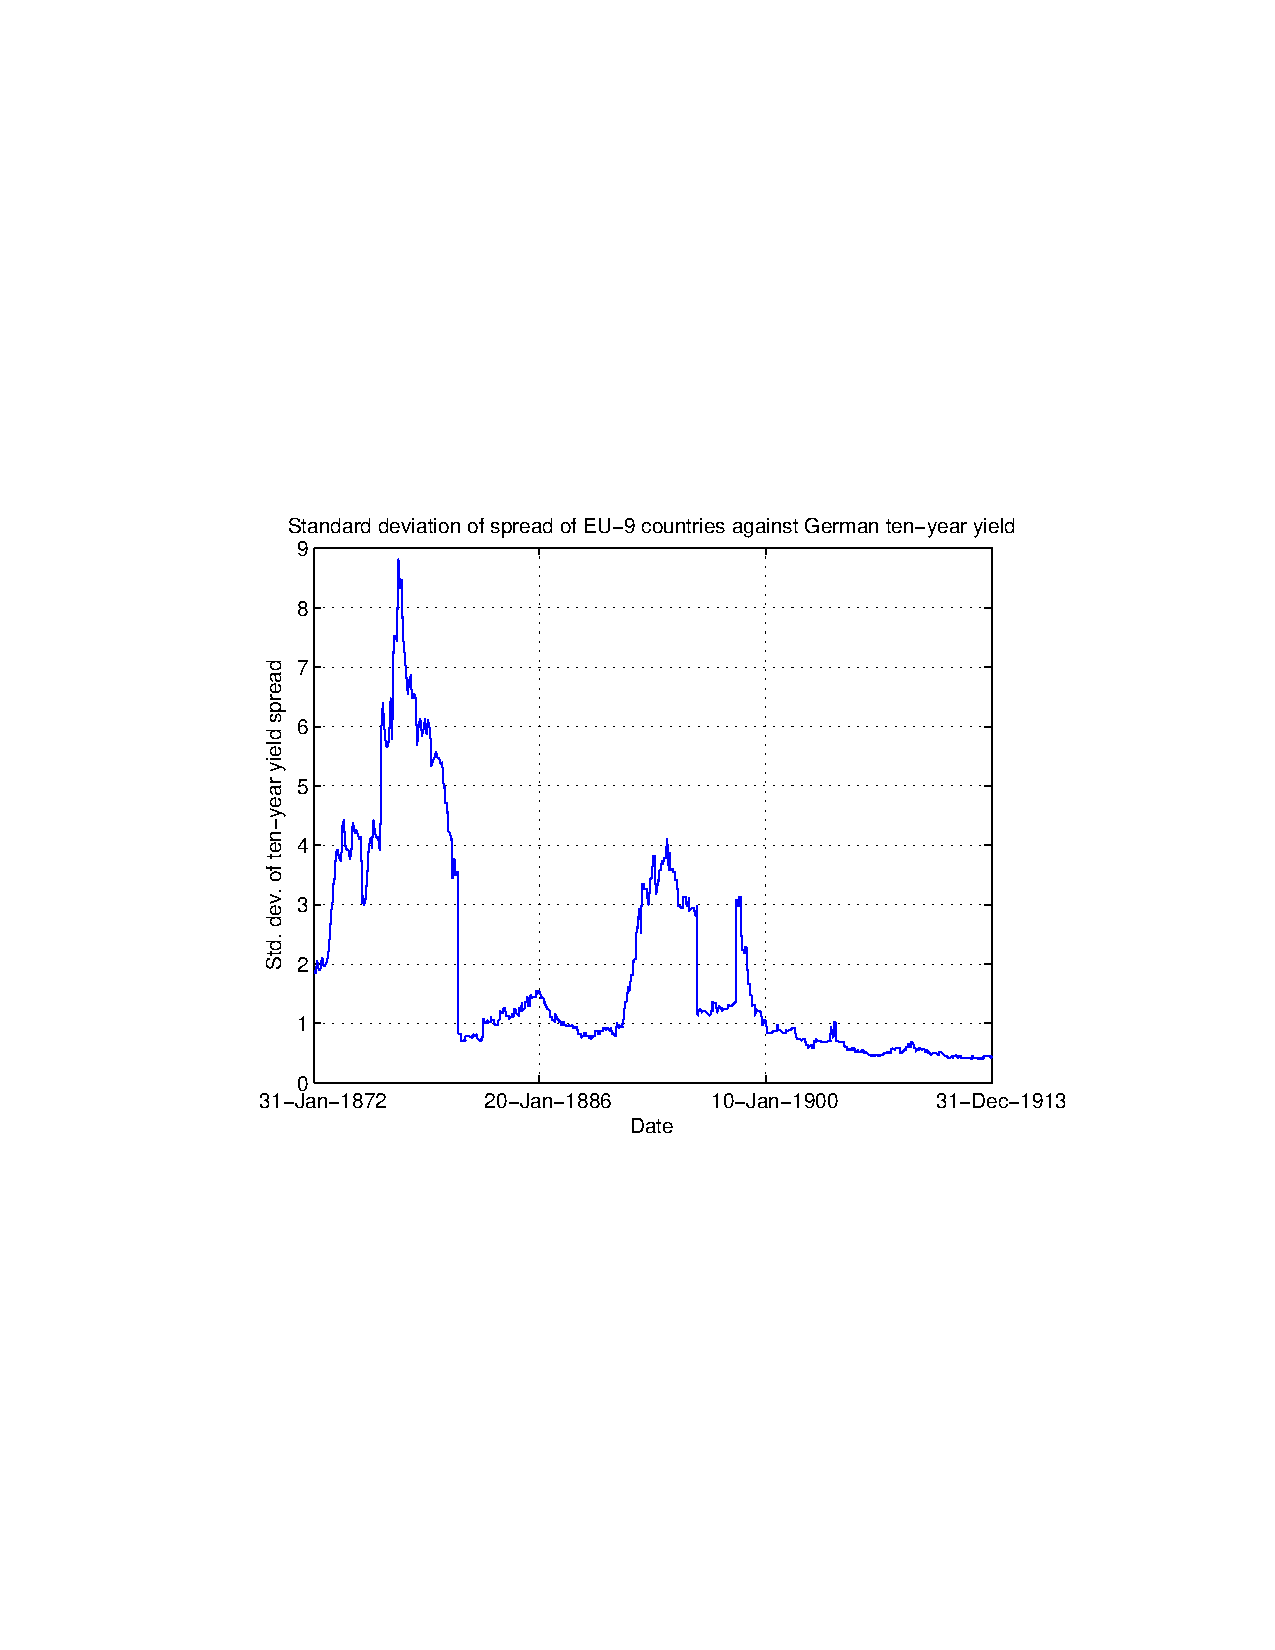
\includegraphics[width=7cm]{fig_de_stdspread_eu9}\\
	\end{tabular}
	\caption{(a) Top, country-specific spread, (b) Bottom left, mean spread, and (c) Bottom right, standard deviation of spread of EU-9 countries against German ten-year yield, 1872-1913.}
	\label{fig:de_spread_eu9}
\end{figure}

Figure \ref{fig:maxeig_eu9} displays (a) the maximum eigenvalue and (b) standard deviation of the leading eigenvector for the correlation in yields.  In this sample, there is a slightly positive trend in the maximum eigenvalue ($0.0061 \cdot year - 7.3$) and a slightly negative trend in the standard deviation of the leading eigenvector ($-0.0024 \cdot year + 4.8$, slope term same sign at two s.e.).  At its peak, the maximum  eigenvalue indicates that 75\% of the variance is explained by the first component, whereas the sample mean is 47\%.

Figure \ref{fig:diff_maxeig_eu9} displays (a) the maximum eigenvalue and (b) standard deviation of the leading eigenvector for the correlation in the first-order difference of yields.  For these differences, the maximum eigenvalue is decreasing over the sample ($-0.015 \cdot year + 32$) and the standard deviation of the leading eigenvector is increasing ($0.0016 \cdot year - 2.8$, slope term same sign at two s.e.)

\begin{figure}[ht!]
	\centering
	\begin{tabular}{cc}
		\includegraphics[width=7cm]{fig_maxeig_eu9} & \includegraphics[width=7cm]{fig_maxeigstd_eu9}
	\end{tabular}
	\caption{(a) Left, maximum eigenvalue and (b) Right, standard deviation of leading eigenvector of correlation of ten-year yields within the EU-9 member countries, 1872-1913.}
	\label{fig:maxeig_eu9}
\end{figure}

\begin{figure}[ht!]
	\centering
	\begin{tabular}{cc}
		\includegraphics[width=7cm]{fig_diff_maxeig_eu9} & 	\includegraphics[width=7cm]{fig_diff_maxeigstd_eu9}
	\end{tabular}
	\caption{(a) Left, maximum eigenvalue and (b) Right, standard deviation of leading eigenvector of correlation of ten-year yields first-difference within the EU-9 member countries, 1872-1913.}
	\label{fig:diff_maxeig_eu9}
\end{figure}

These results seems conflicting at first.  This apparent discrepancy is an example of the improved understanding we can obtain from this method.  While the correlation of actual yields, the specific quoted percent rate, appears increasingly integrated, the correlation of the changes in these yields has become less integrated.  In this sense, we can interpret these findings as follows - though European countries' rates all converge near the German rate over time, their relative changes as they approach this rate become decreasingly dependent.  In summary, though these markets appear to be integrated from the analysis of yield spreads, this more sophisticated analysis reveals that the movement of these yields are decreasingly correlated over the period.

\subsection{EU-12: 1958-2010}
Figure \ref{fig:de_spread_eu12} displays a summary of the sovereign bond yield spread relative to German bonds for the period from 1958 to 2010.  Panel (a) plots each country's spread over the period.  There are a number of points to note in this figure.  First, until the period surrounding the expansion of the European Community, the collapse of Bretton Woods, and the oil crisis of the 1970s, the German yield was actually higher than most other European sovereign yields.  Only after these events did the German yield become the benchmark.  Second, the volatility of these yields has gone through a number of very distinct regimes.  The period of extremely low volatility between 1995 and 2007 is also worth highlighting.  

In general, the absolute value of the mean spread against the German yield has fallen over this period, from approximately 2\% at the outset of the sample to just under 1\% in the final year.  During the late 1990s and early 2000s, these spreads were very close to zero.  However, the hyperinflation and oil crisis of the 1970s drove yield spreads as high as 7\%, and the recent global and Eurozone crises has driven these yields substantially higher than zero.  The standard deviation of spreads confirms these interpretation.

\begin{figure}[ht!]
	\centering
	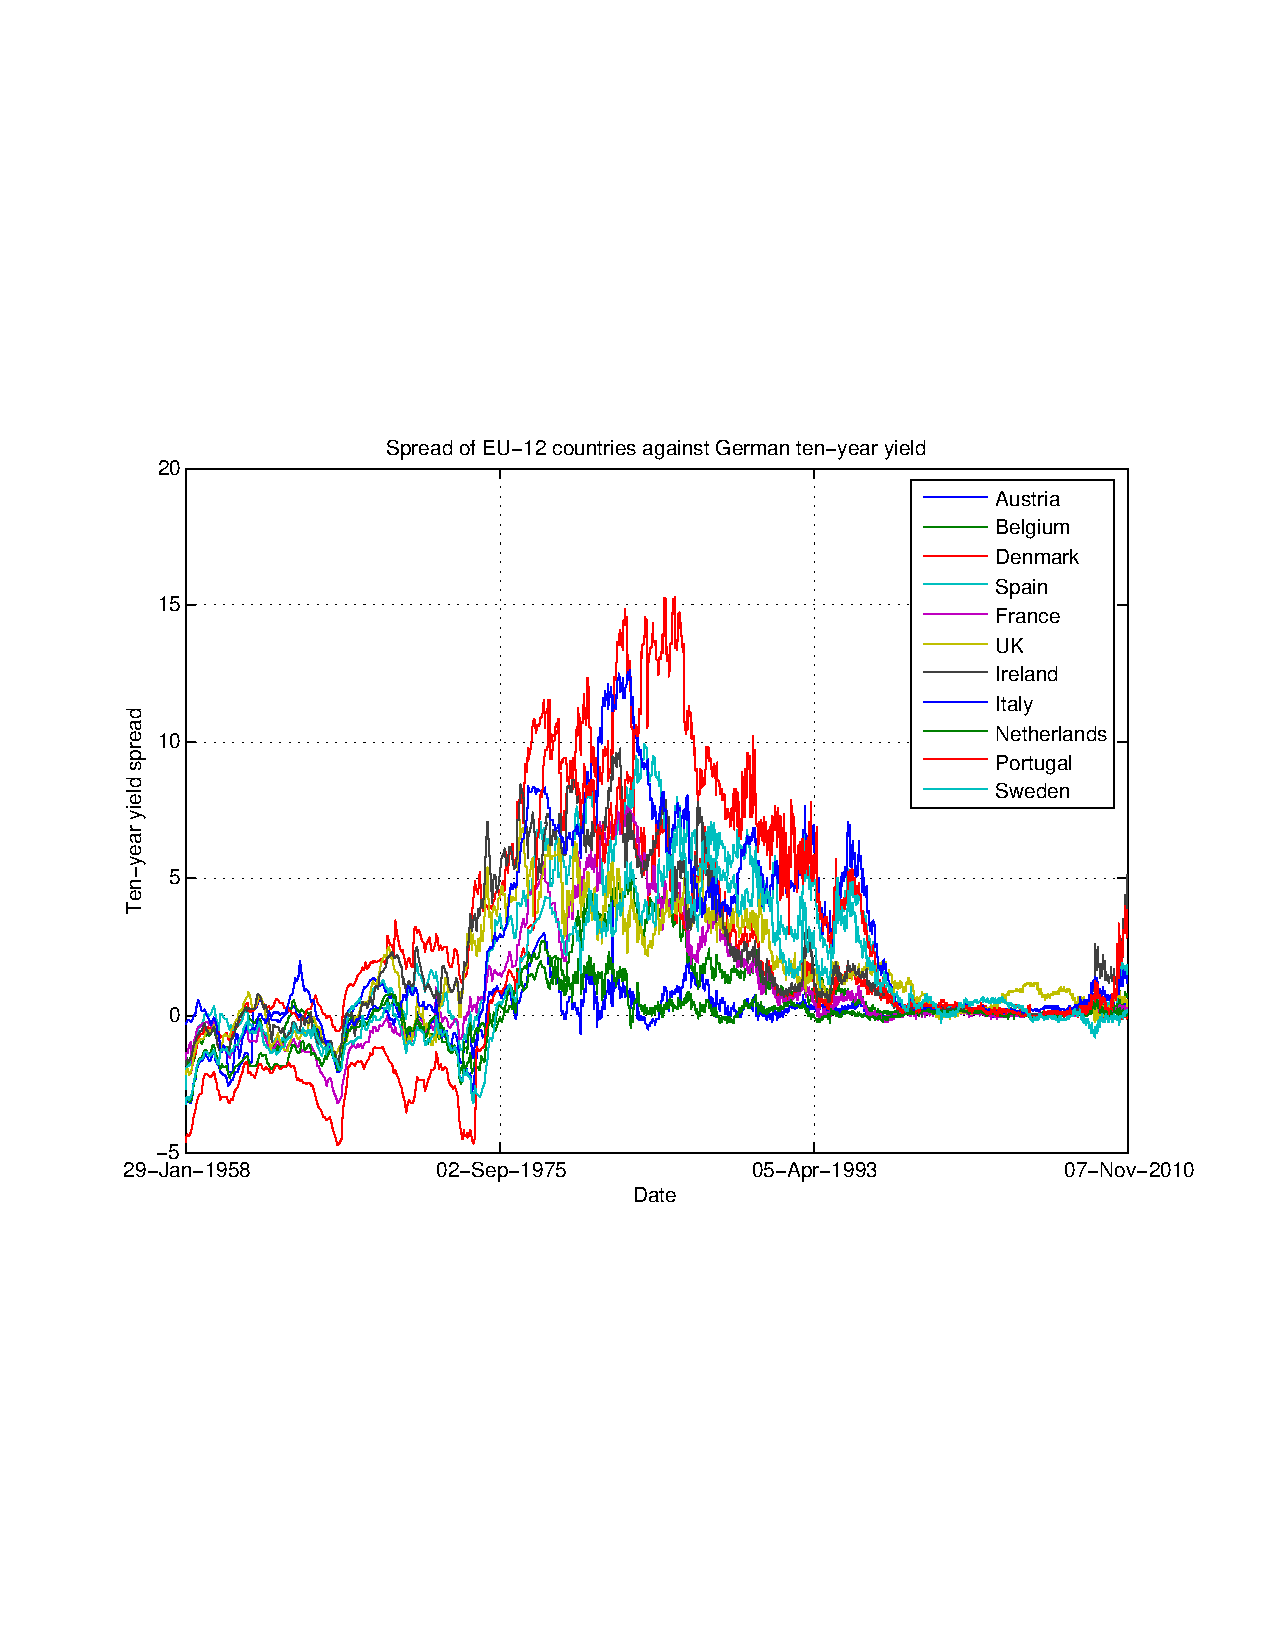
\includegraphics[width=9cm]{fig_de_spread_eu12}
	\begin{tabular}{cc}
		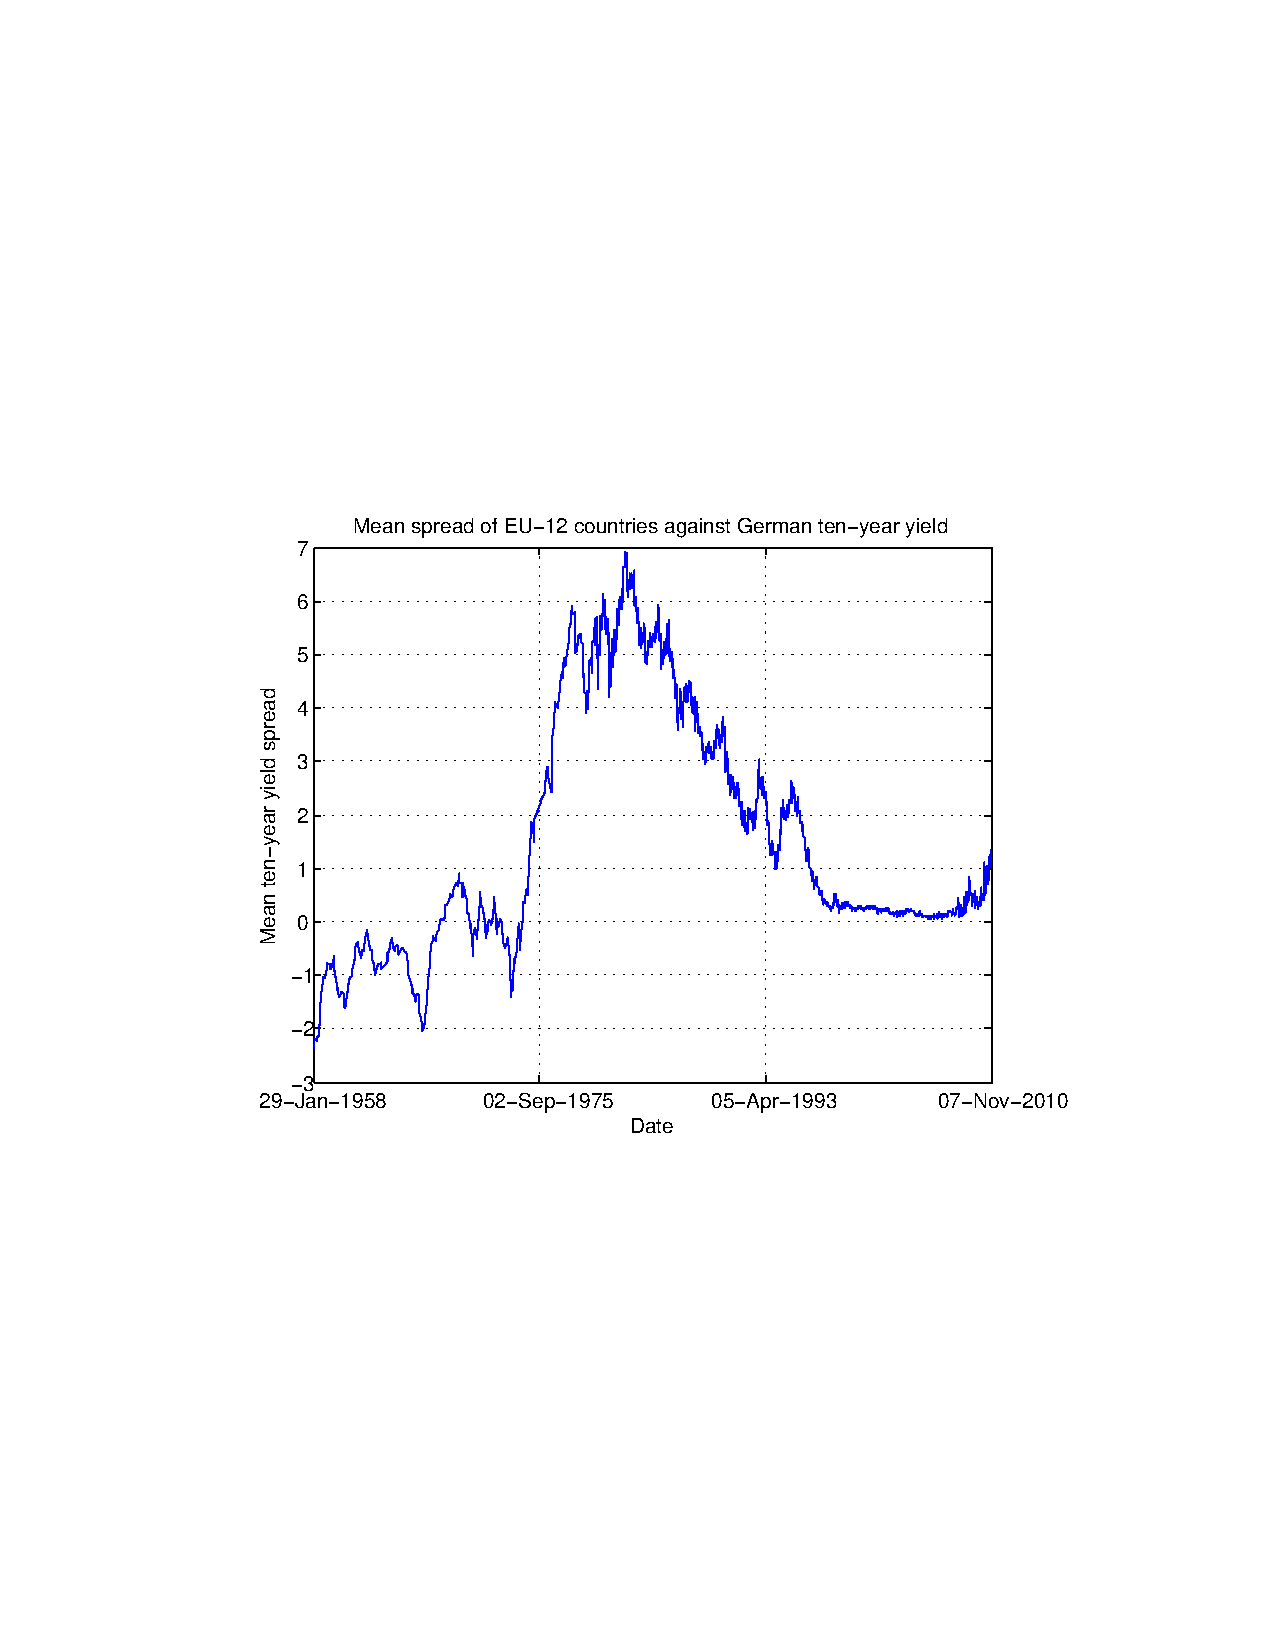
\includegraphics[width=7cm]{fig_de_meanspread_eu12} & 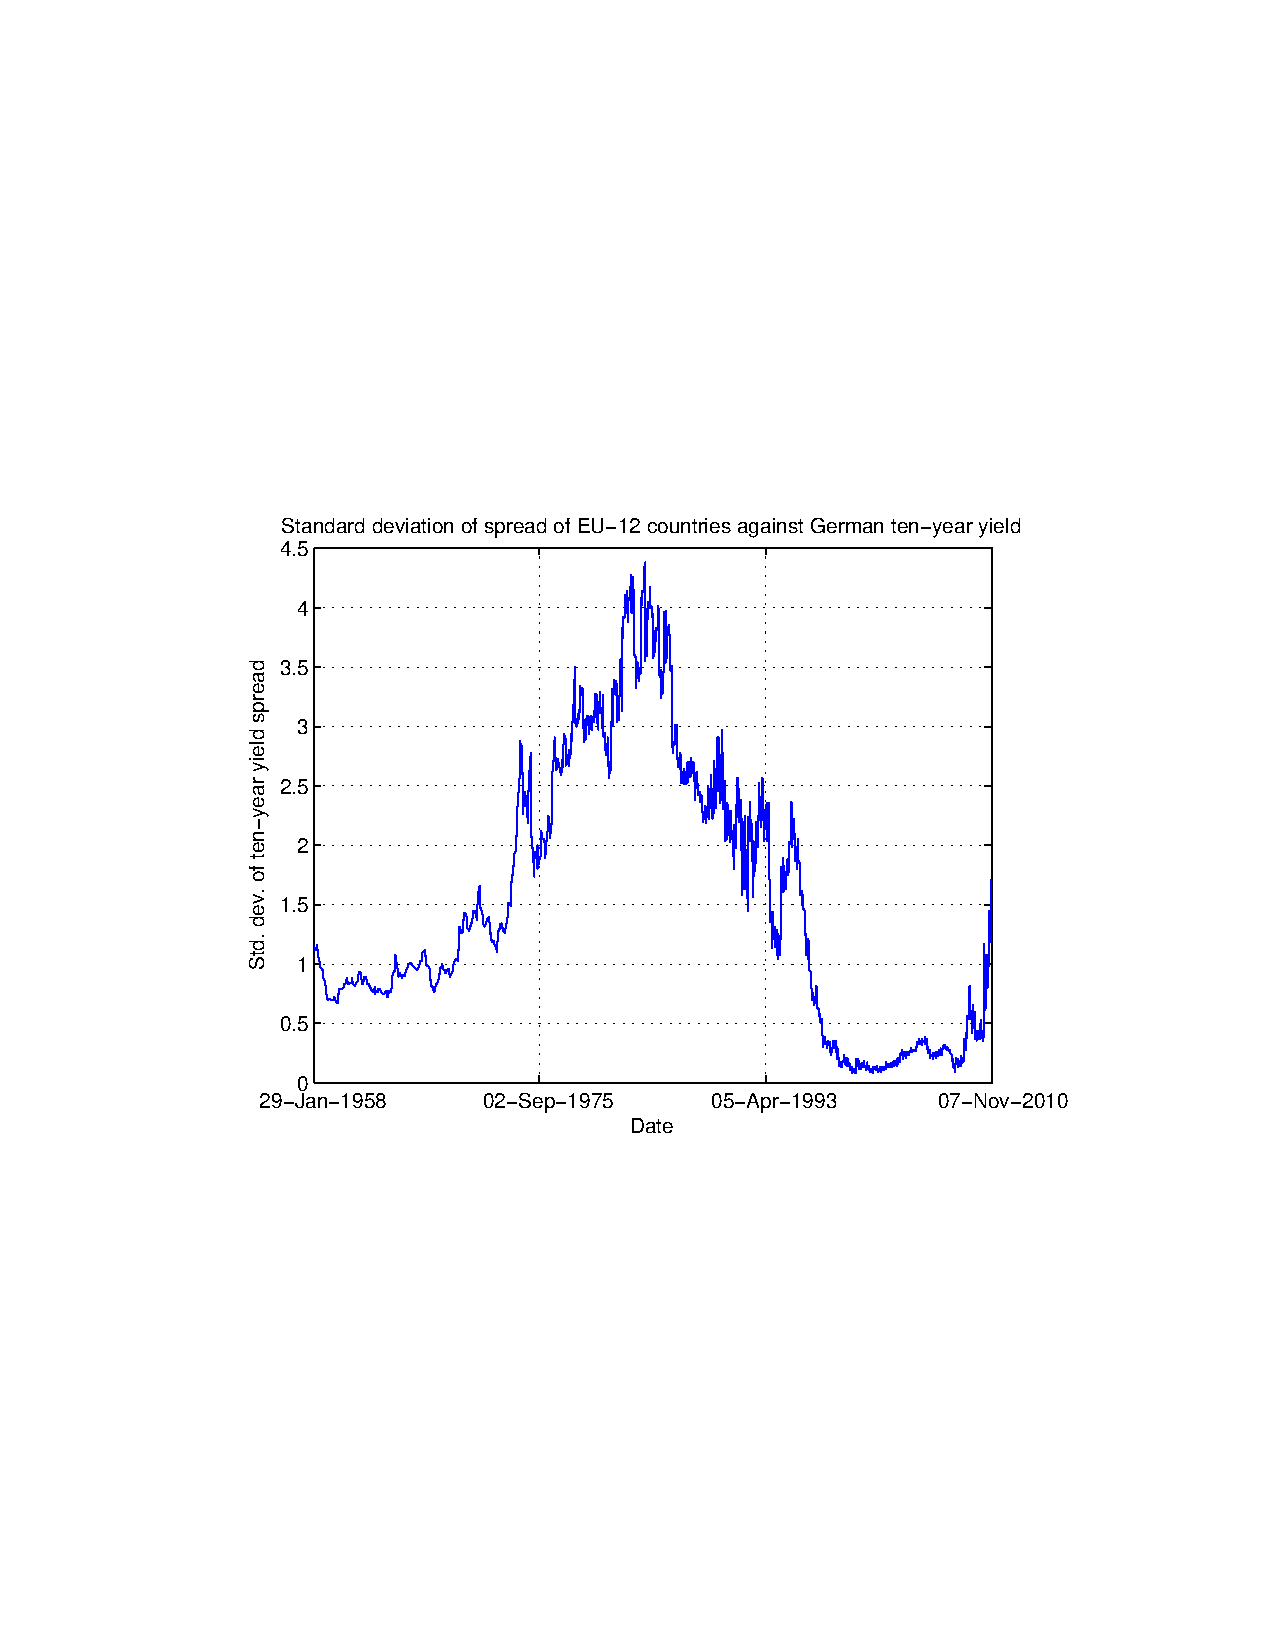
\includegraphics[width=7cm]{fig_de_stdspread_eu12}\\
	\end{tabular}
	\caption{(a) Top, country-specific spread, (b) Bottom left, mean spread, and (c) Bottom right, standard deviation of spread of EU-12 countries against German ten-year yield, 1958-2010.}
	\label{fig:de_spread_eu12}
\end{figure}


Figure \ref{fig:maxeig_eu12} displays (a) the maximum eigenvalue and (b) standard deviation of the leading eigenvector for the correlation in yields.  In this sample, there is a strong positive trend in the maximum eigenvalue ($0.099 \cdot year - 190$) and a strong negative trend in the standard deviation of the leading eigenvector ($-0.0051 \cdot year + 10$, slope term same sign at two s.e.).  At its peak, the maximum  eigenvalue indicates that 99\% of the variance is explained by the first component, with a sample mean of 69\%.

Figure \ref{fig:diff_maxeig_eu12} displays (a) the maximum eigenvalue and (b) standard deviation of the leading eigenvector for the correlation in the first-order difference of yields.  For these differences, the maximum eigenvalue also exhibits a strongly positive trend ($0.12 \cdot year - 230$) and the standard deviation of the leading eigenvector is rapidly decreasing ($-0.0056 \cdot year + 11$, slope term same sign at two s.e.)

\begin{figure}[ht!]
	\centering
	\begin{tabular}{cc}
		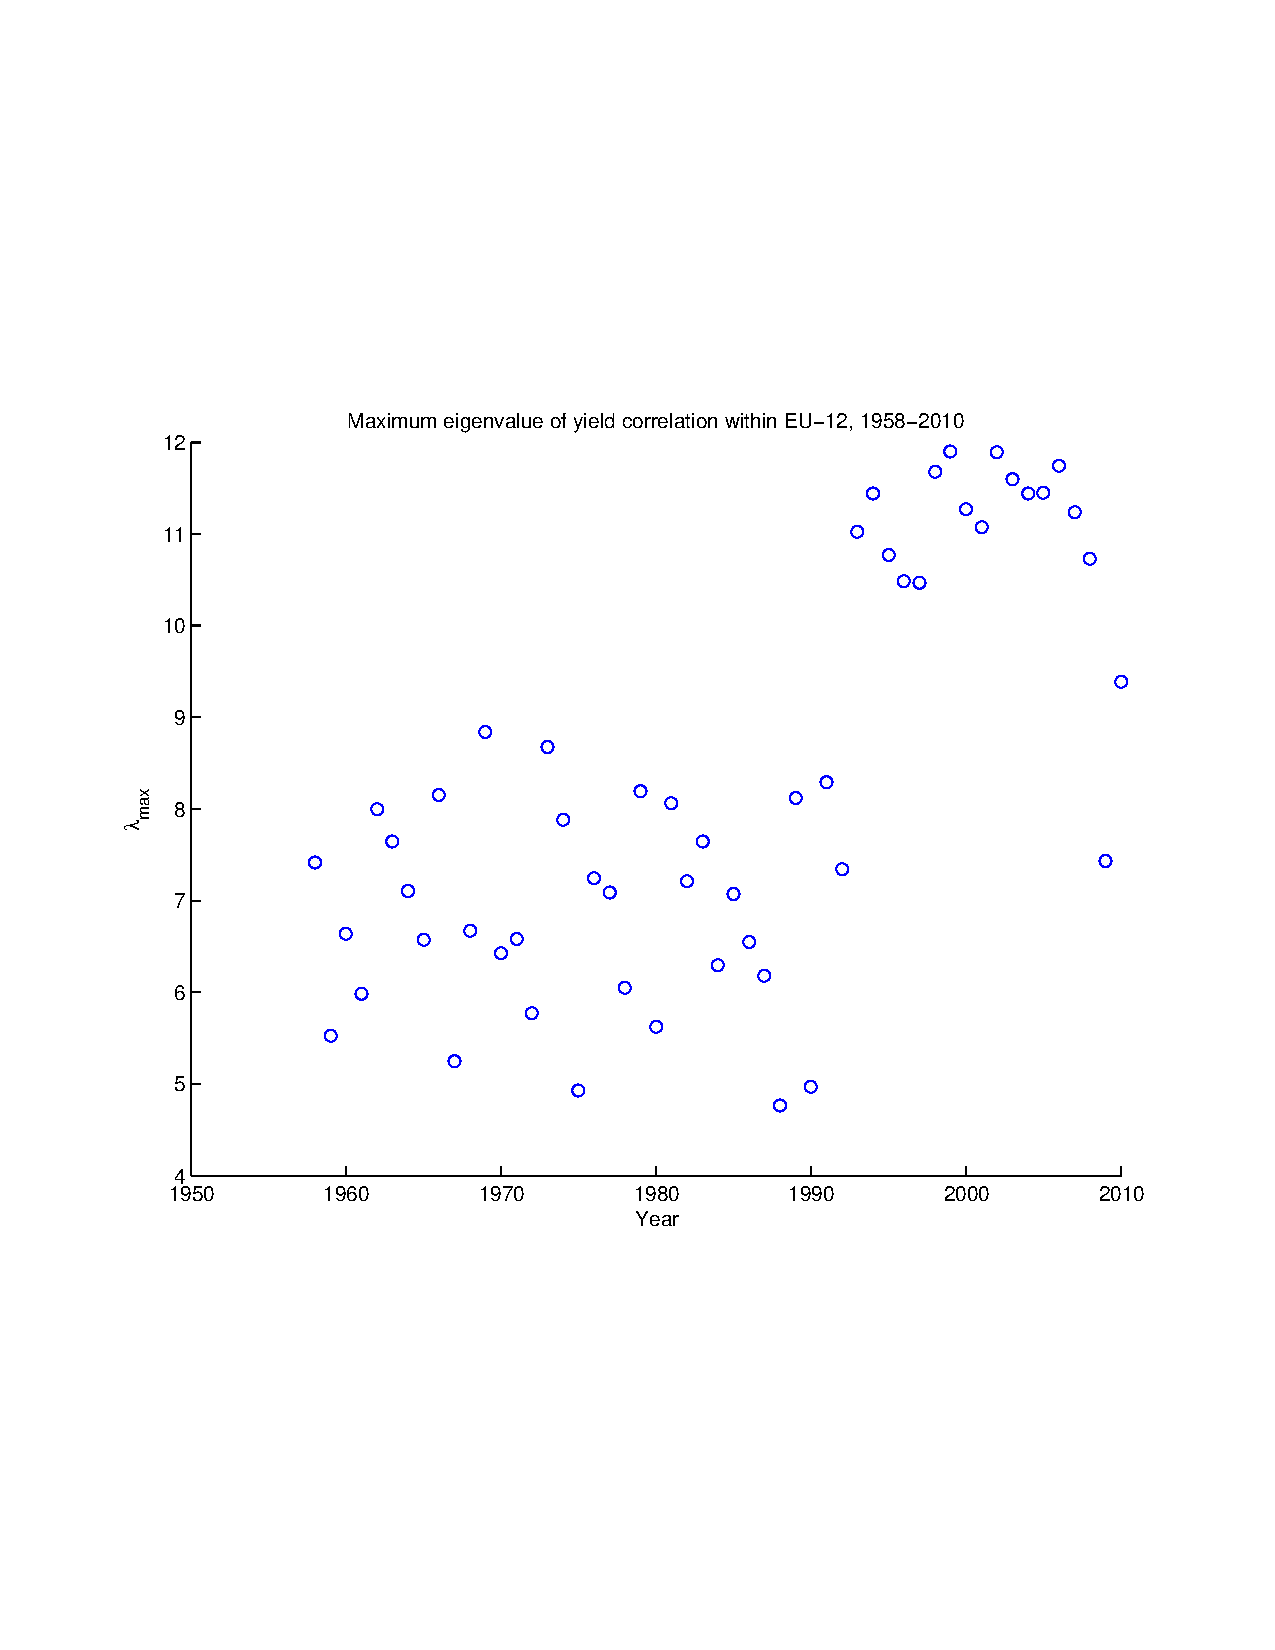
\includegraphics[width=7cm]{fig_maxeig_eu12} & 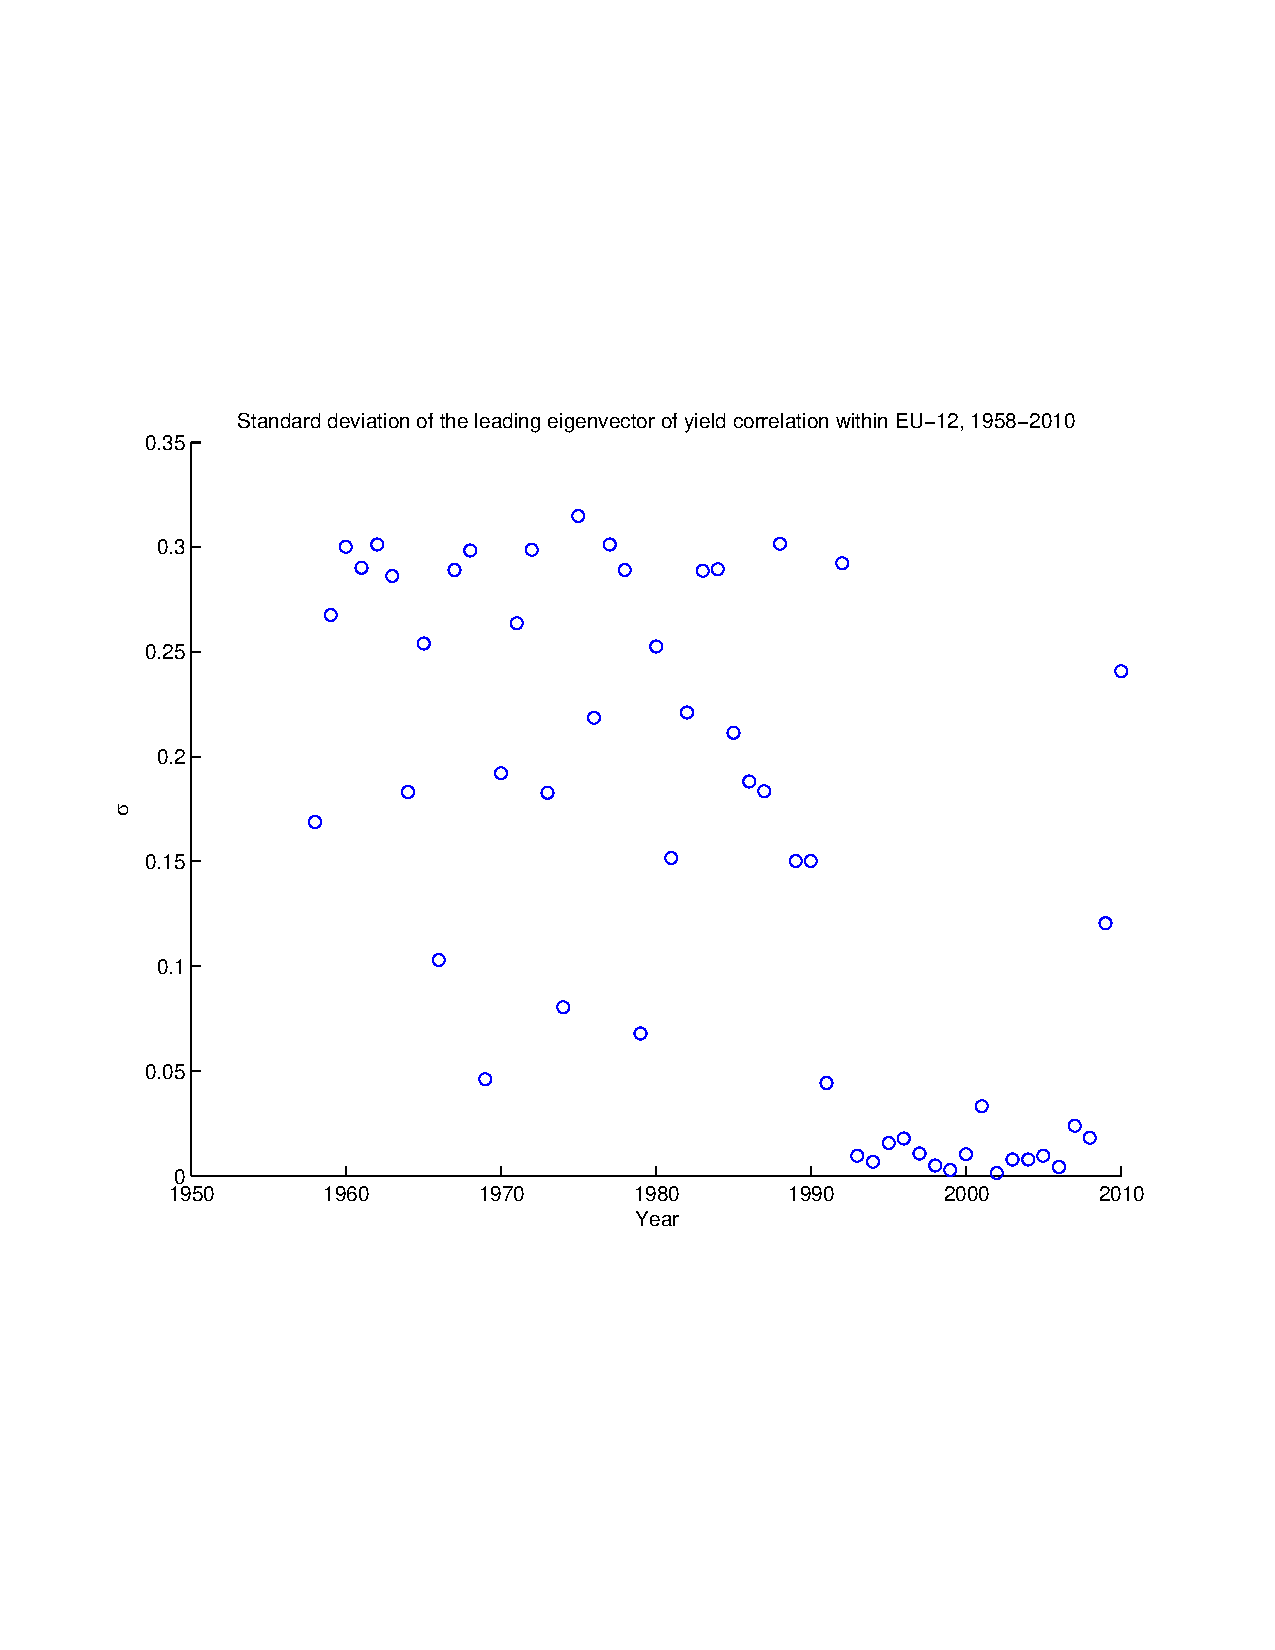
\includegraphics[width=7cm]{fig_maxeigstd_eu12}
	\end{tabular}
	\caption{(a) Left, maximum eigenvalue and (b) Right, standard deviation of leading eigenvector of correlation of ten-year yields within the EU-12 member countries, 1958-2010.}
	\label{fig:maxeig_eu12}
\end{figure}

\begin{figure}[ht!]
	\centering
	\begin{tabular}{cc}
		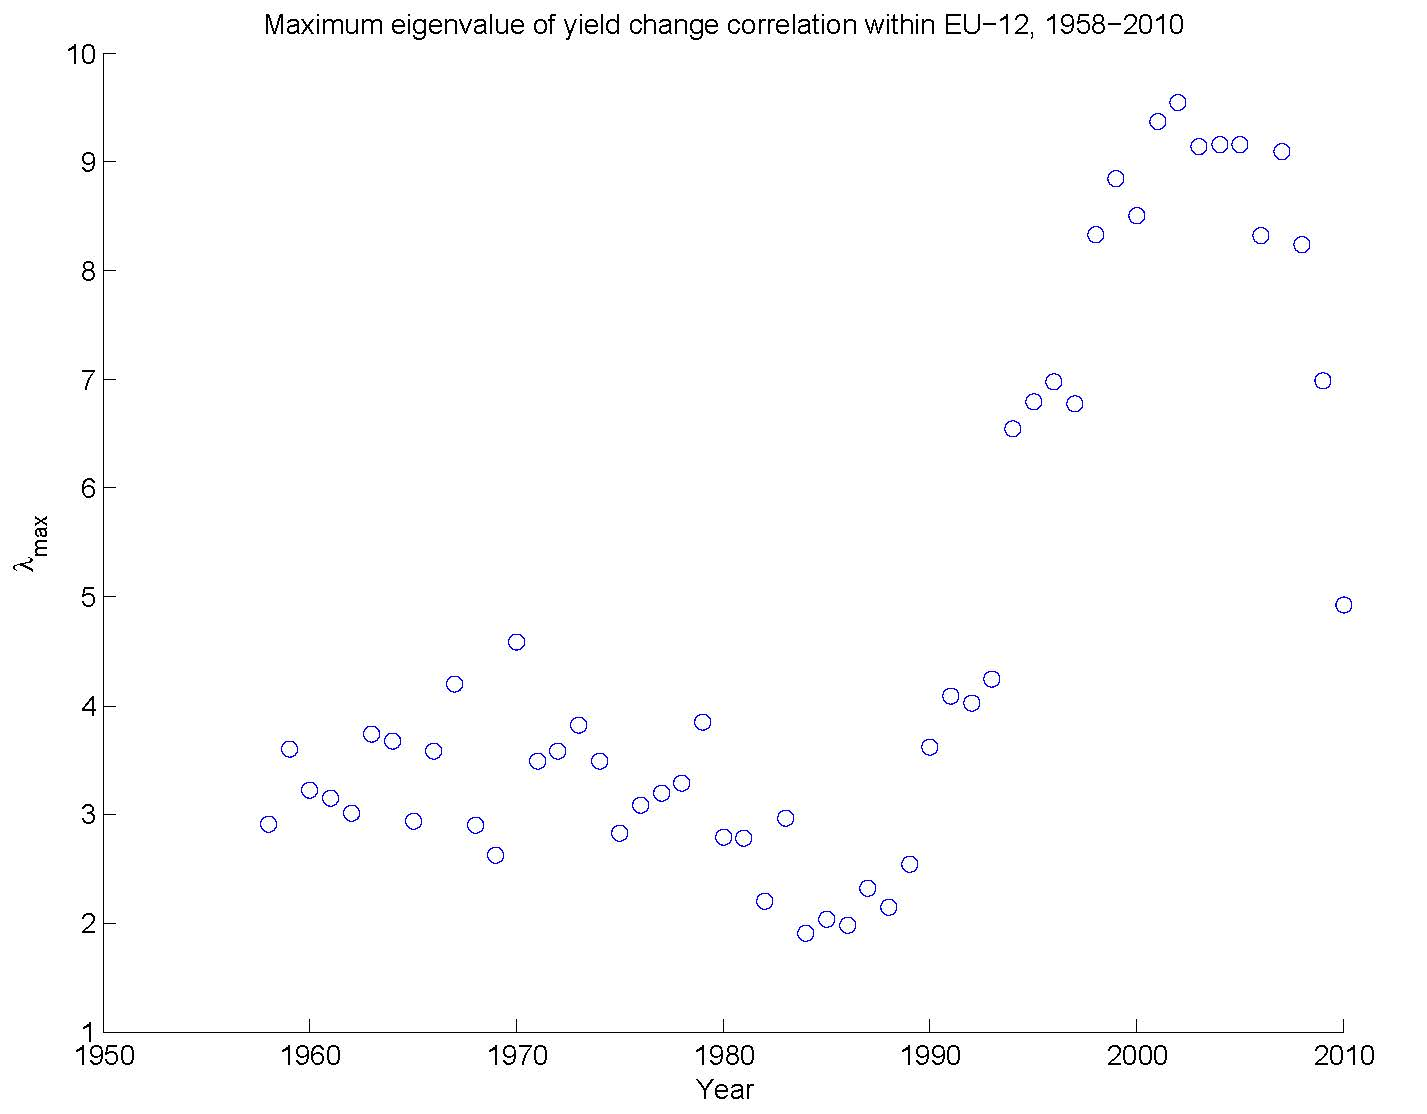
\includegraphics[width=7cm]{fig_diff_maxeig_eu12} & 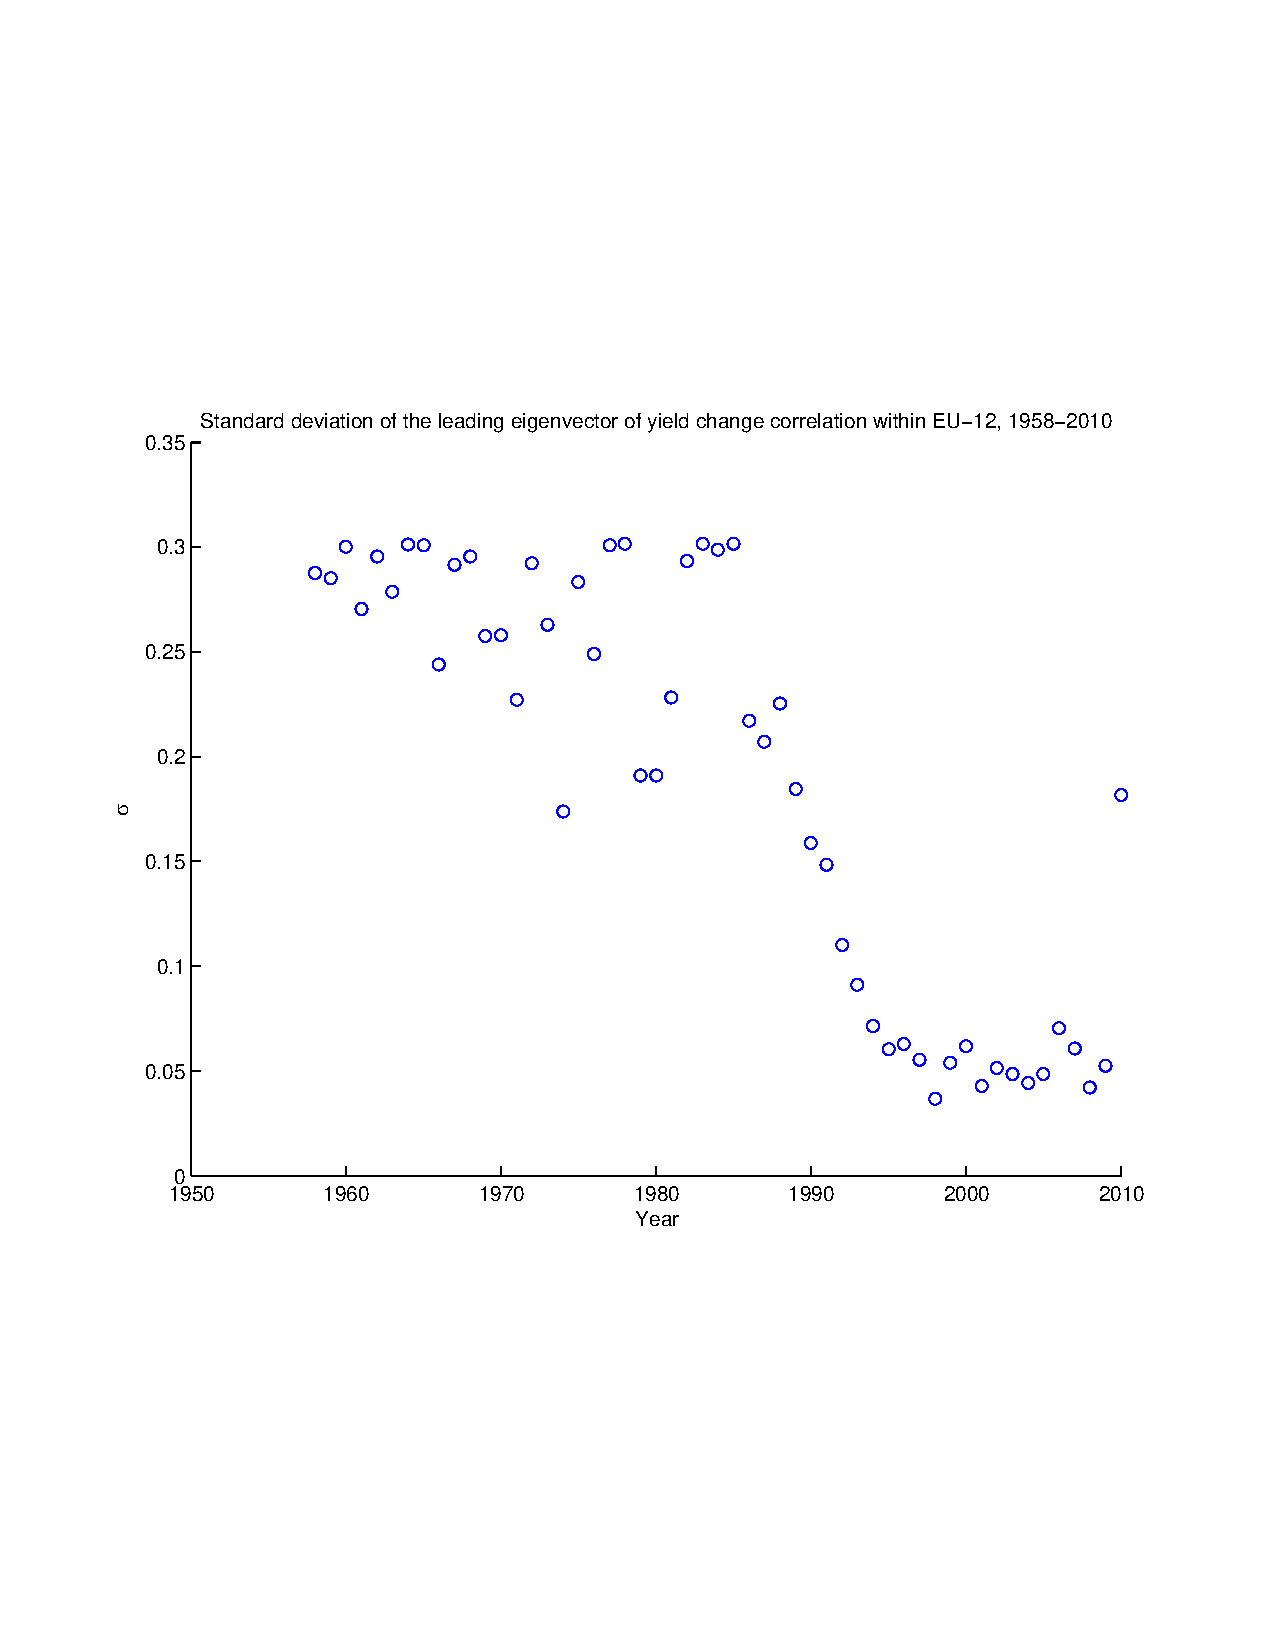
\includegraphics[width=7cm]{fig_diff_maxeigstd_eu12}
	\end{tabular}
	\caption{(a) Left, maximum eigenvalue and (b) Right, standard deviation of leading eigenvector of correlation of ten-year yields first-difference within the EU-12 member countries, 1958-2010.}
	\label{fig:diff_maxeig_eu12}
\end{figure}

As opposed to the EU-9 sample above, we see that the spectral decompositions of correlation for both the yield and first-order difference of yield agree.  The maximum eigenvalue is strongly increasing over the sample period and the standard deviation of the leading eigenvector is strongly decreasing.  With the exception of 2009 and 2010, in which these values returned to pre-Maastricht levels, the Euro sovereign bond market appears to have seen strong integration over this period.  

Hidden in figures \ref{fig:maxeig_eu12} and \ref{fig:diff_maxeig_eu12} are an even more important point.  These spectral measures of integration do not identify the 1970s oil crisis, as opposed to the massive spike demonstrated in the yield spread.  This is because the differences in the yield spread are likely caused by changes in systemic risk and asset volatility, not caused by changes in actual linkage between countries.  This is an important advantage of spectral methods based on correlation matrices over raw yield spreads.

\subsection{EU-15: 1987-2010}
The EU-15 sample is almost identical to the EU-12 dataset; the primary difference is that Finland, Luxembourg, and Greece are included in the EU-15 sample, and that the sample begins in 1987.  Figure \ref{fig:de_spread_eu15} displays a summary of the sovereign bond yield spread relative to German bonds for the period from 1987 to 2010.  Panels (a), (b), and (c) all appear qualitatively identical to the second half of their respective panels in figure \ref{fig:de_spread_eu12}.  The only noticeable difference in panels (b) and (c) is that the mean spread and standard deviation of spread are slightly higher as a result of Greece's inclusion.  Panel (a) clearly shows that the recent Greek crisis is not unique and that Greece has repeatedly suffered fiscal crises that hamper EU integration efforts.

\begin{figure}[ht!]
	\centering
	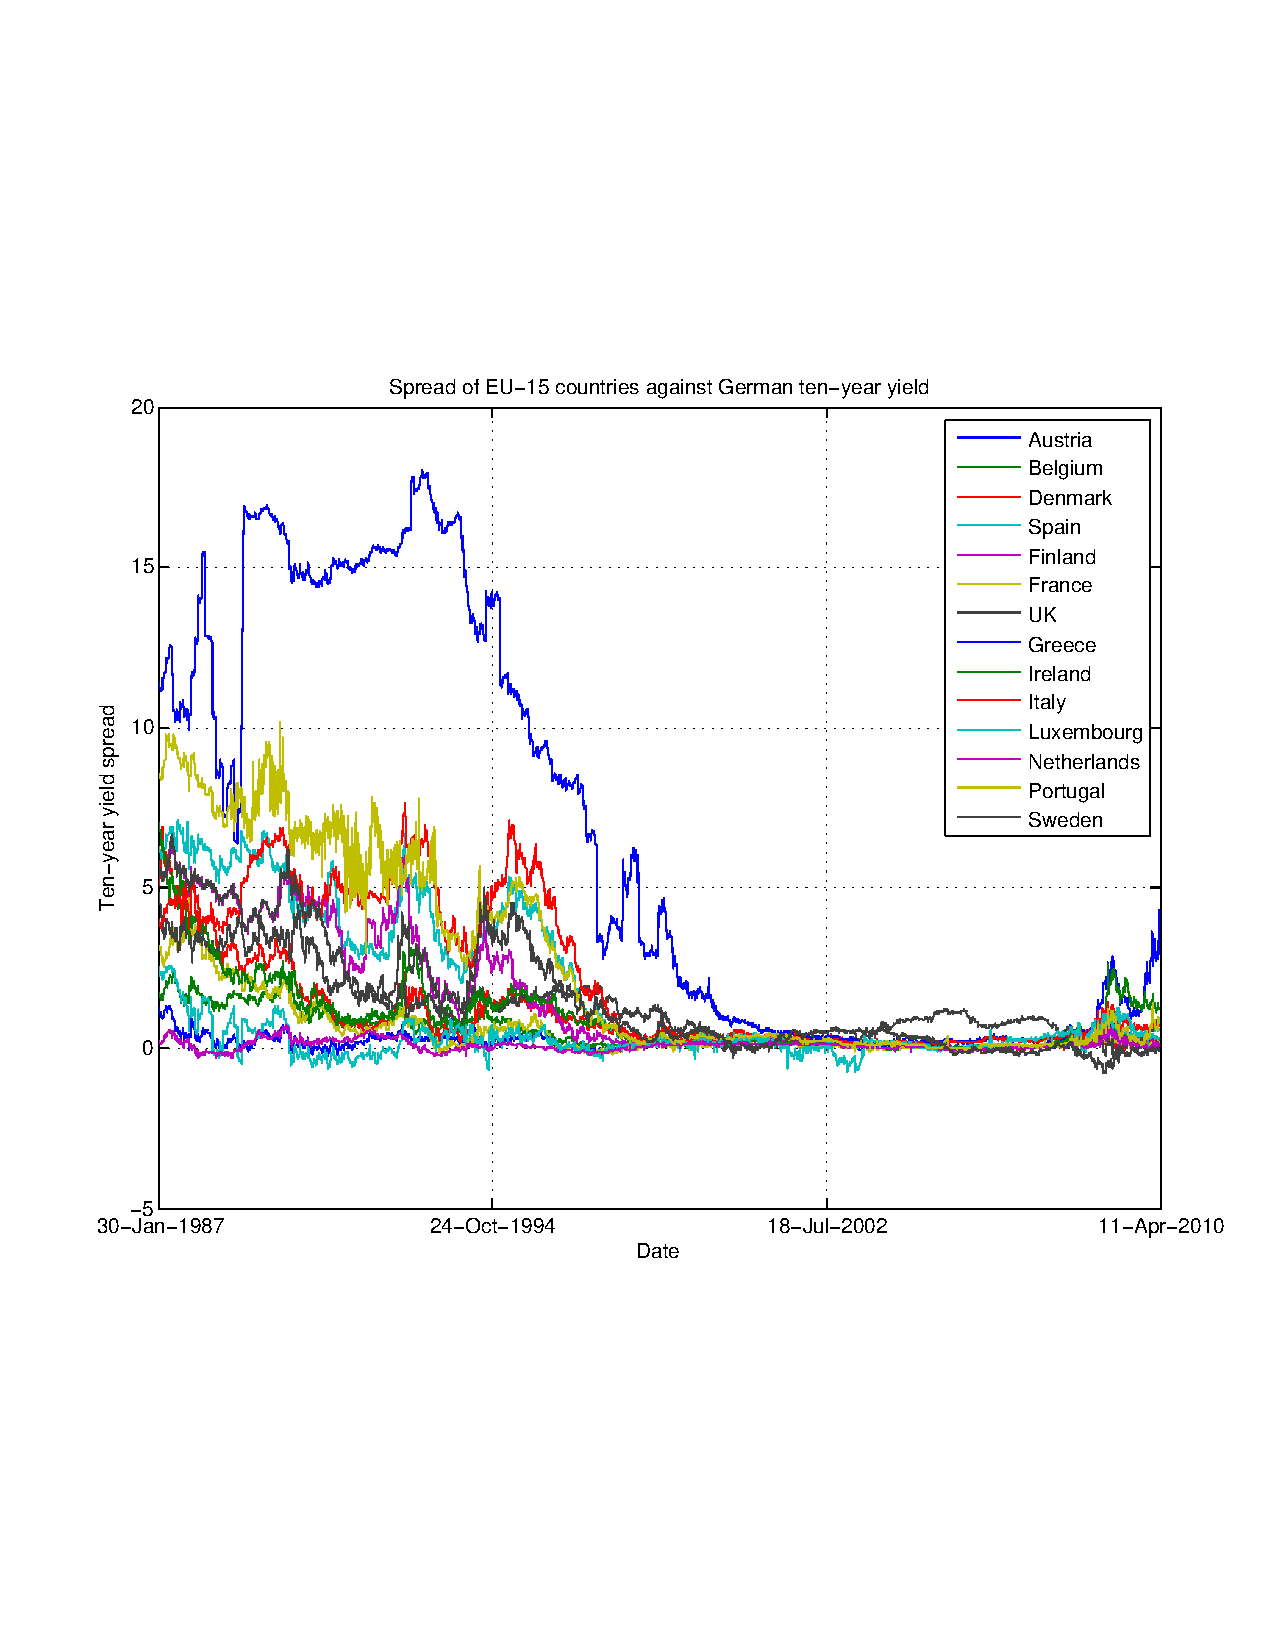
\includegraphics[width=9cm]{fig_de_spread_eu15}
	\begin{tabular}{cc}
		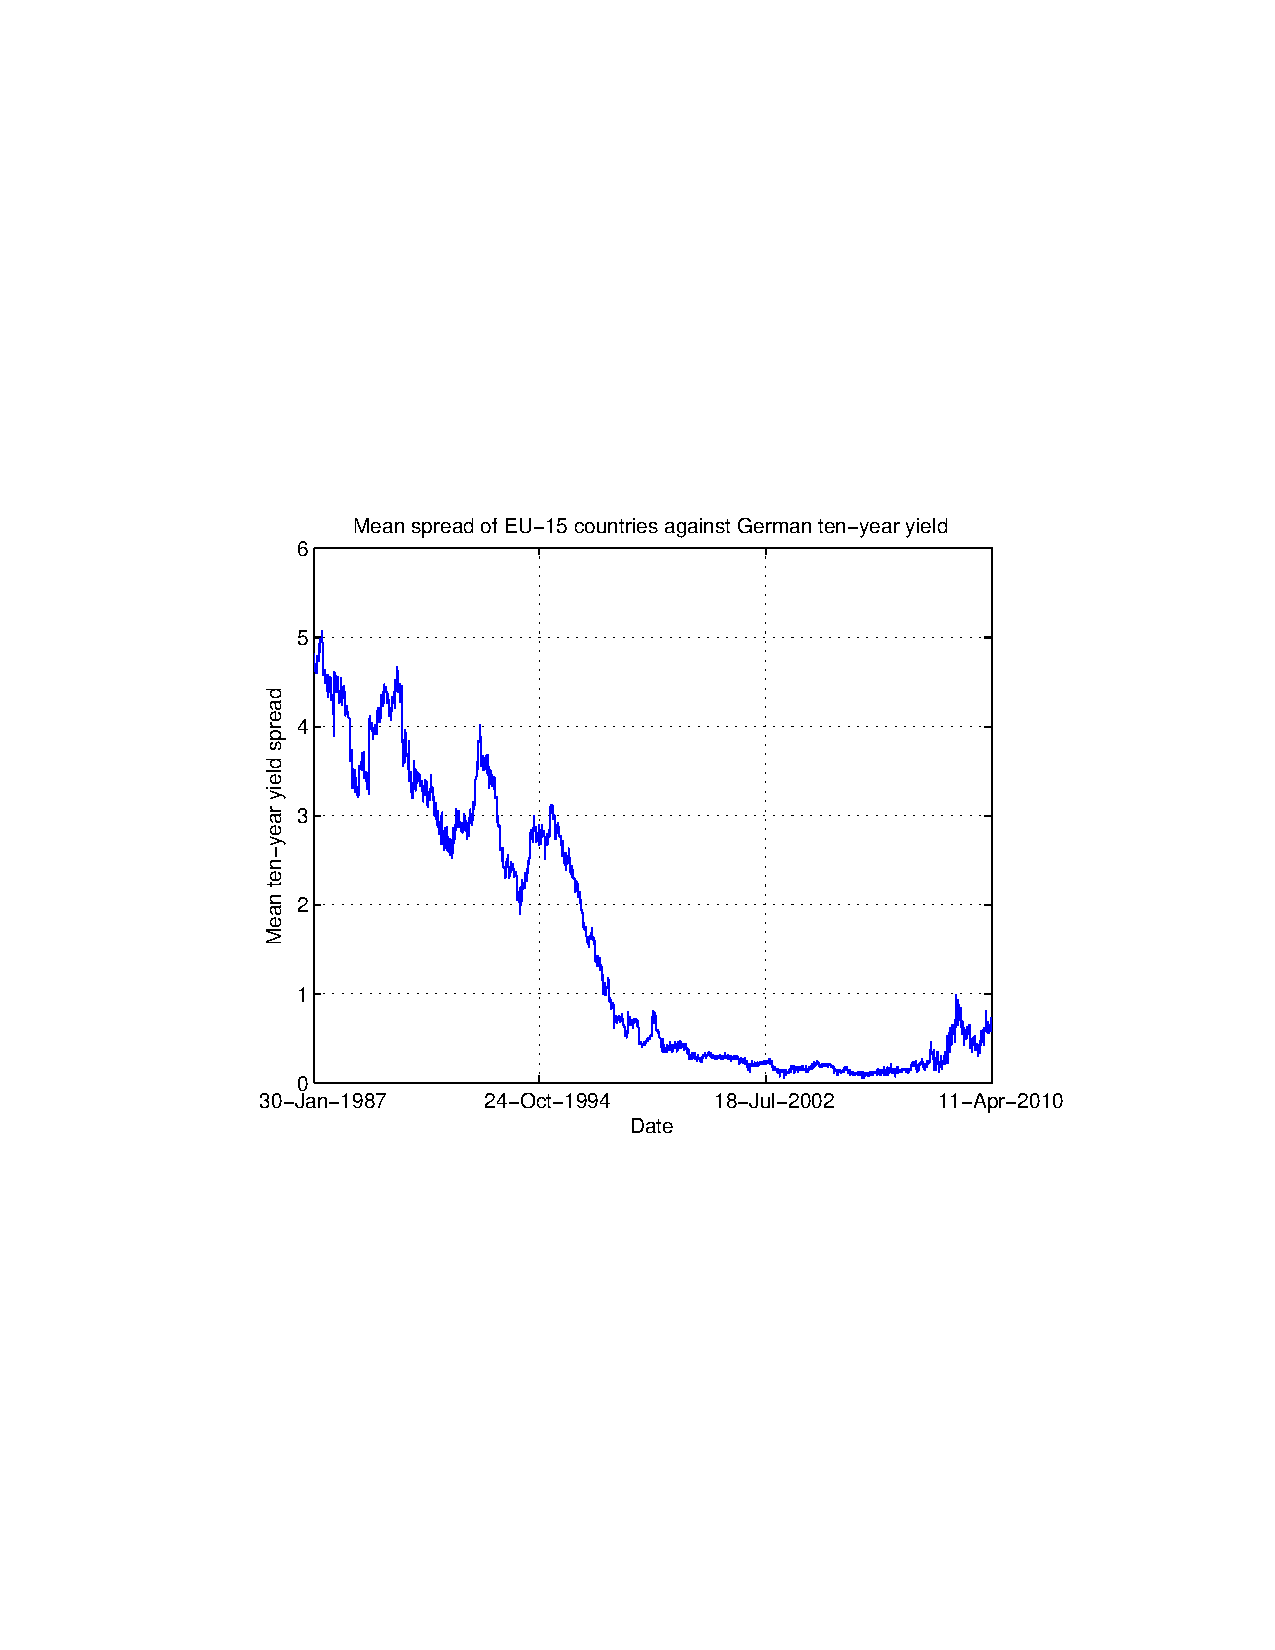
\includegraphics[width=7cm]{fig_de_meanspread_eu15} & 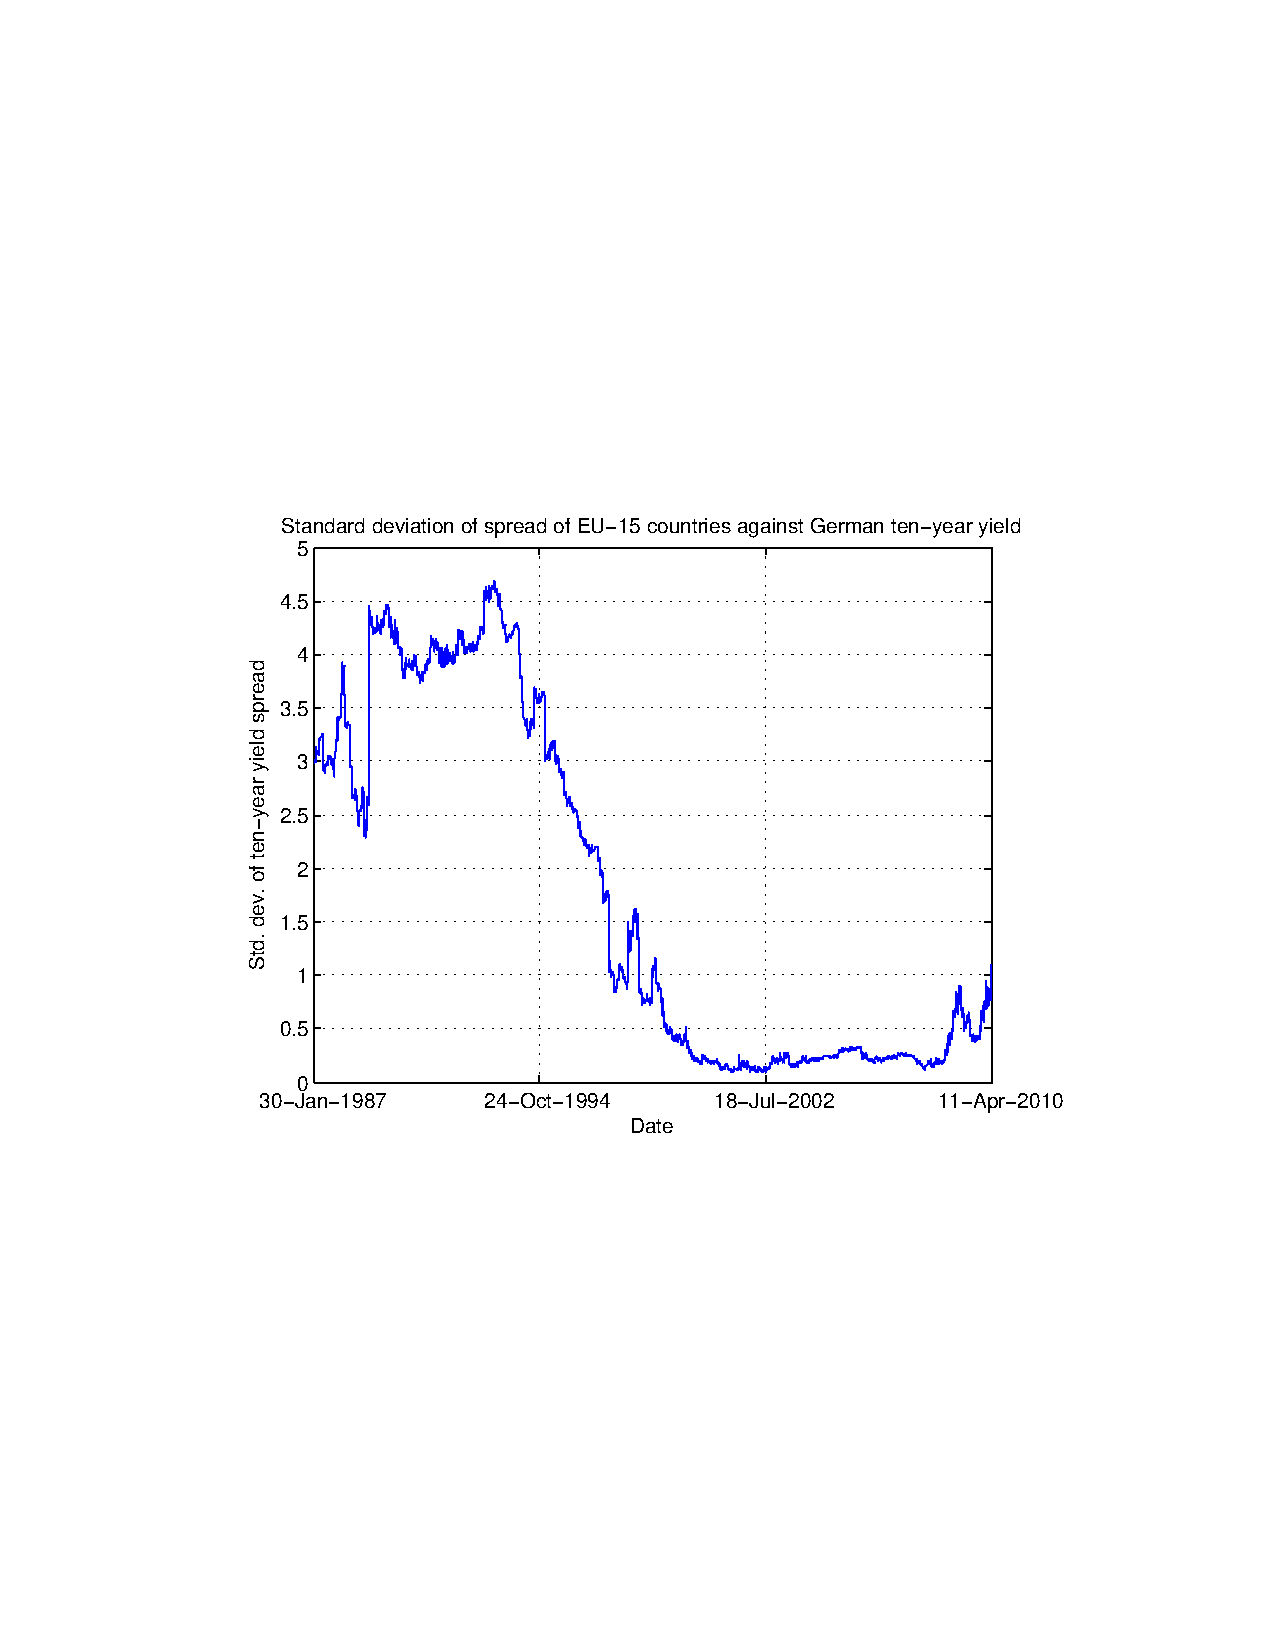
\includegraphics[width=7cm]{fig_de_stdspread_eu15}\\
	\end{tabular}
	\caption{(a) Top, country-specific spread, (b) Bottom left, mean spread, and (c) Bottom right, standard deviation of spread of EU-15 countries against German ten-year yield, 1987-2010.}
	\label{fig:de_spread_eu15}
\end{figure}

Figures \ref{fig:maxeig_eu15} and \ref{fig:diff_maxeig_eu15} are also qualitatively similar to their counterpart figures \ref{fig:maxeig_eu12} and \ref{fig:diff_maxeig_eu12}.  The pre-crisis trend in both yield and first-order difference of yield is strongly towards integration.  However, in this EU-15 sample, the crisis begins to decrease the maximum eigenvalue a year earlier than in the EU-12 sample.  This is again likely the result of the inclusion of Greece.

\begin{figure}[ht!]
	\centering
	\begin{tabular}{cc}
		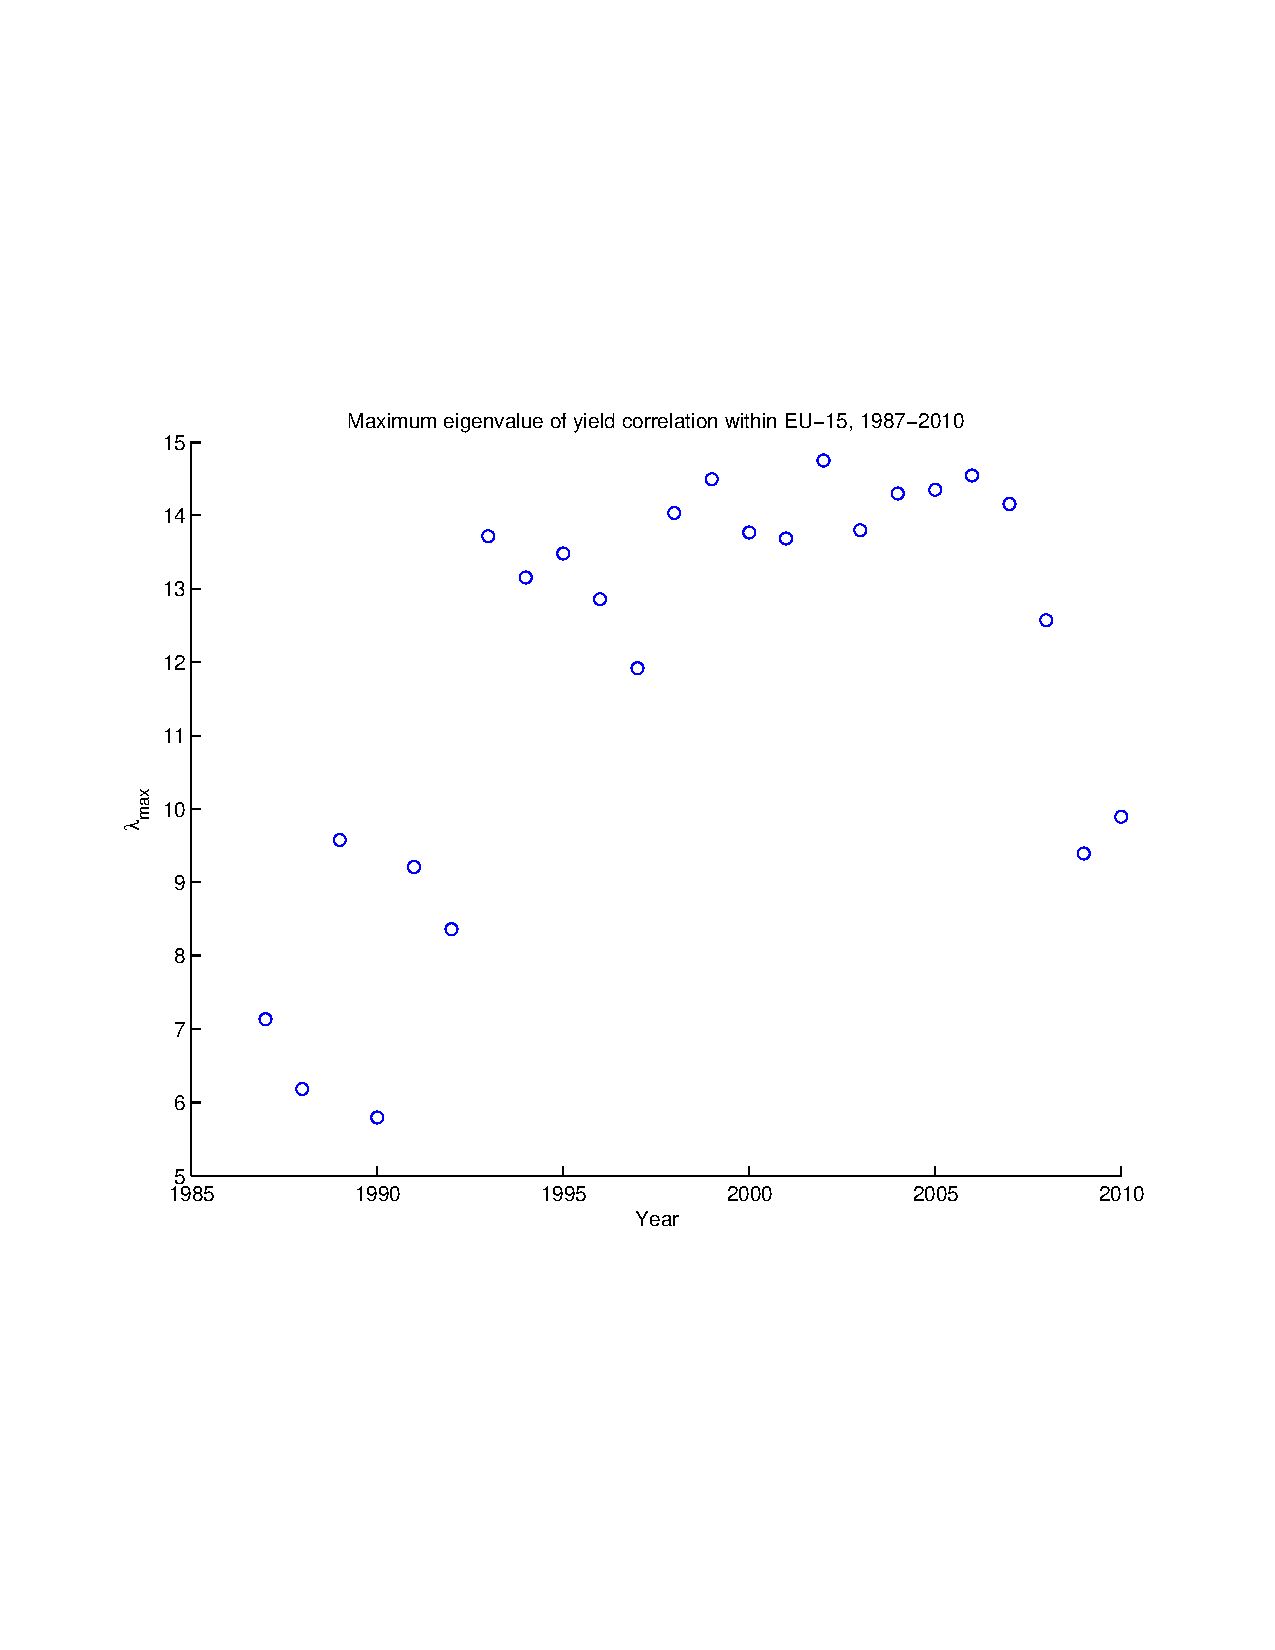
\includegraphics[width=7cm]{fig_maxeig_eu15} & 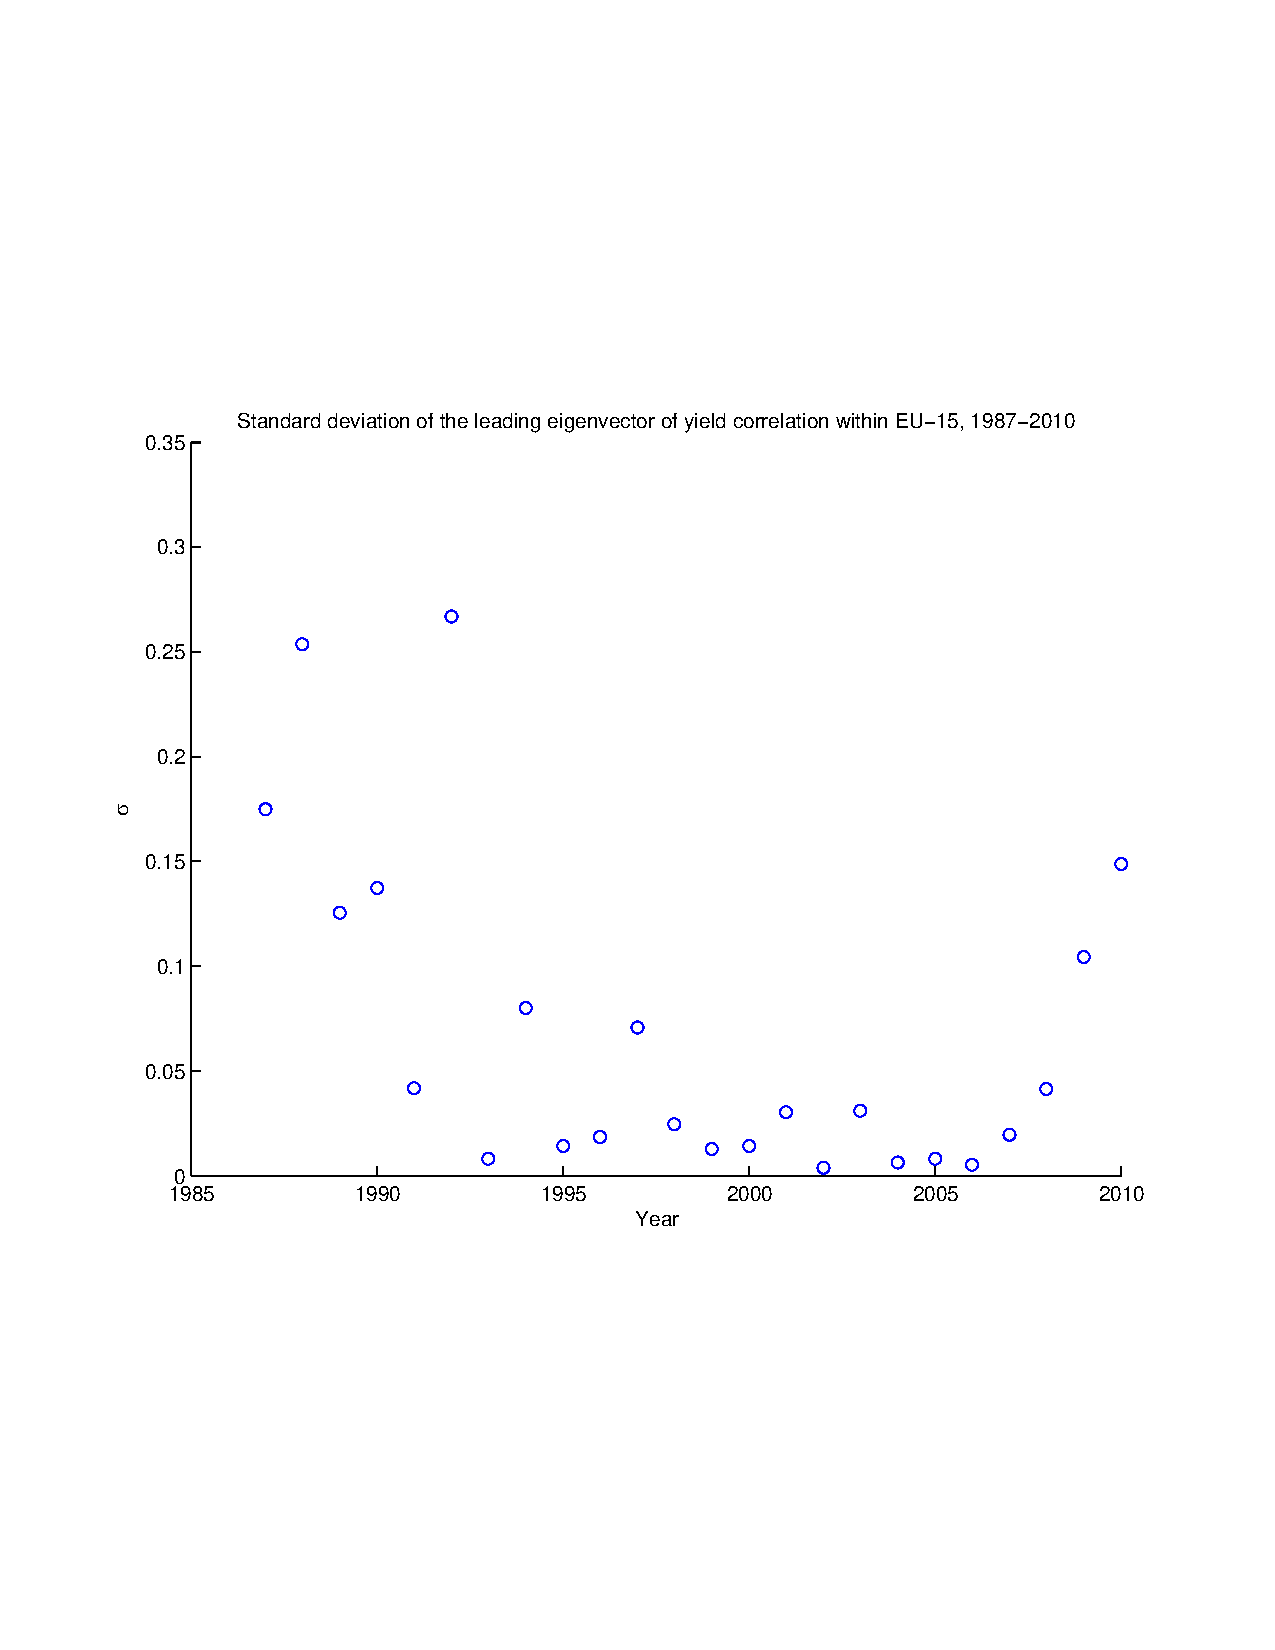
\includegraphics[width=7cm]{fig_maxeigstd_eu15}
	\end{tabular}
	\caption{(a) Left, maximum eigenvalue and (b) Right, standard deviation of leading eigenvector of correlation of ten-year yields within the EU-15 member countries, 1987-2010.}
	\label{fig:maxeig_eu15}
\end{figure}

\begin{figure}[ht!]
	\centering
	\begin{tabular}{cc}
		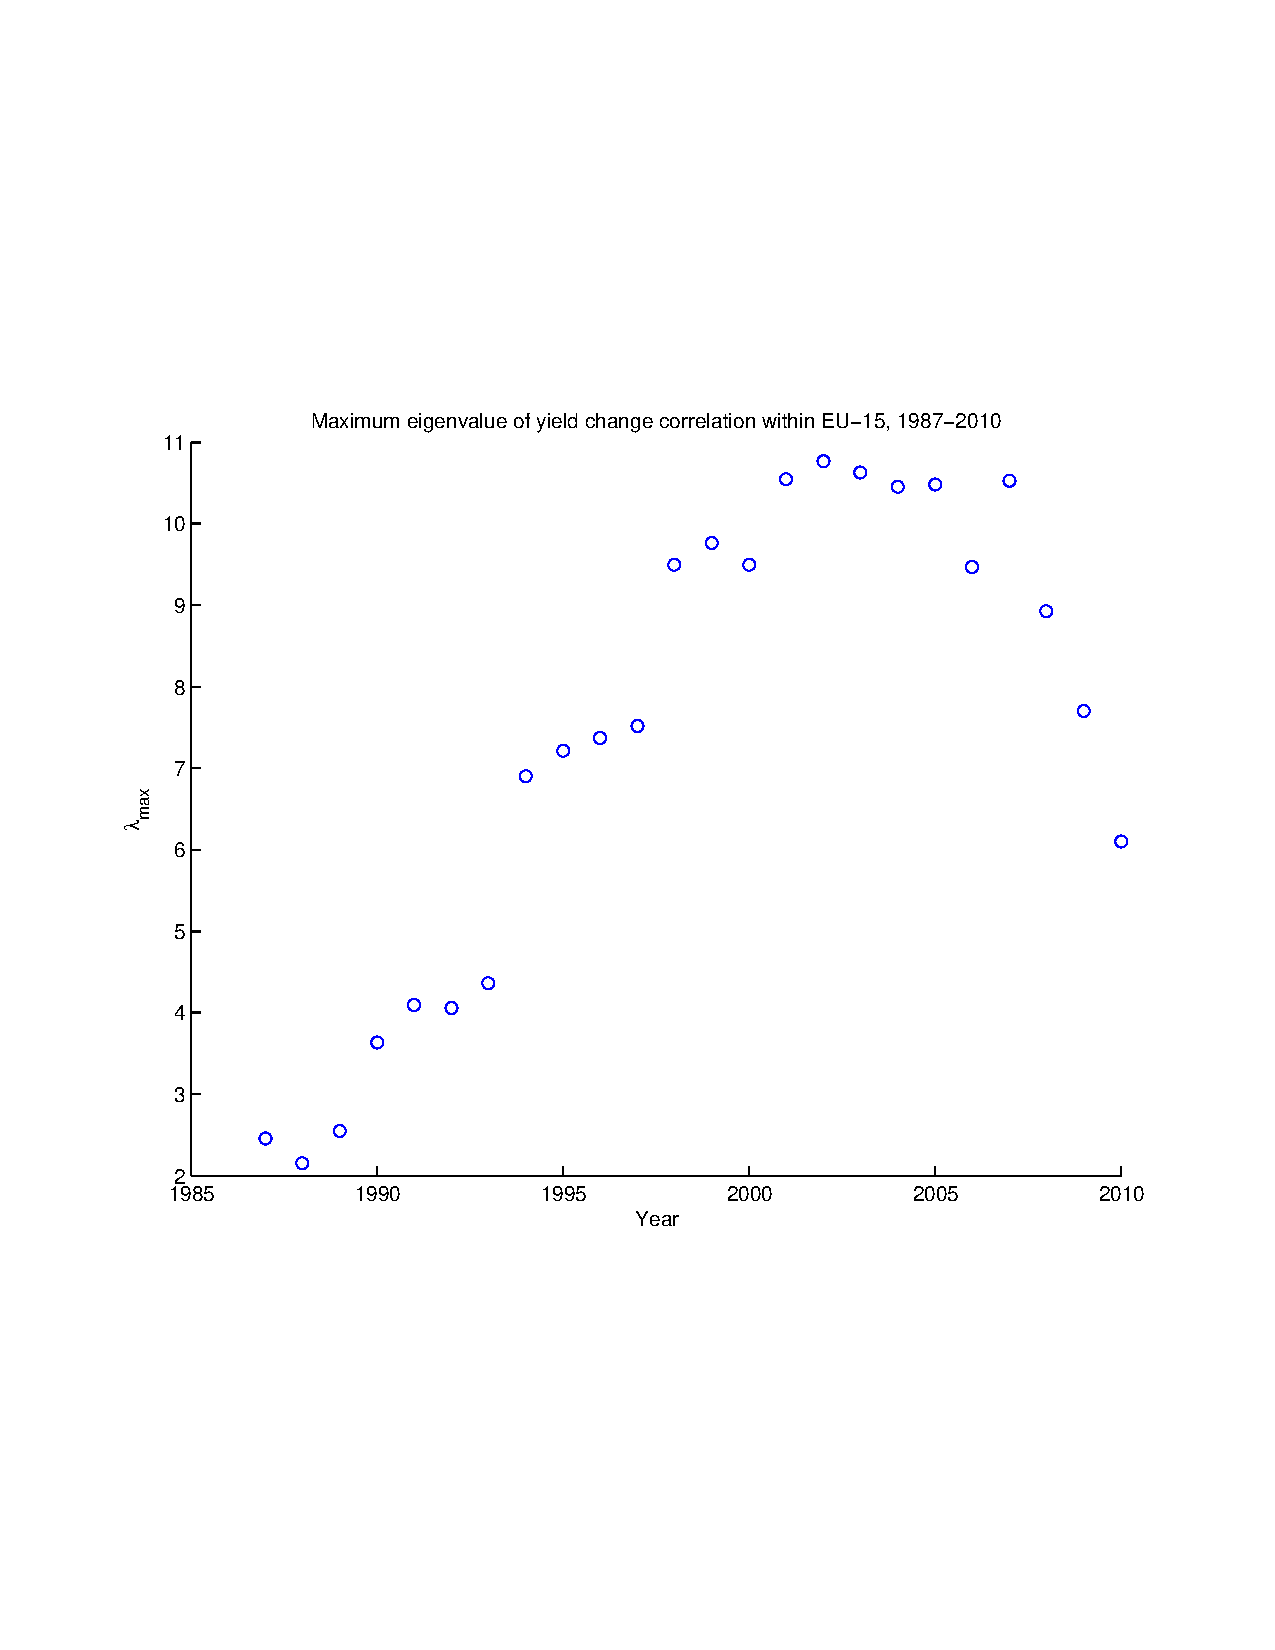
\includegraphics[width=7cm]{fig_diff_maxeig_eu15} & 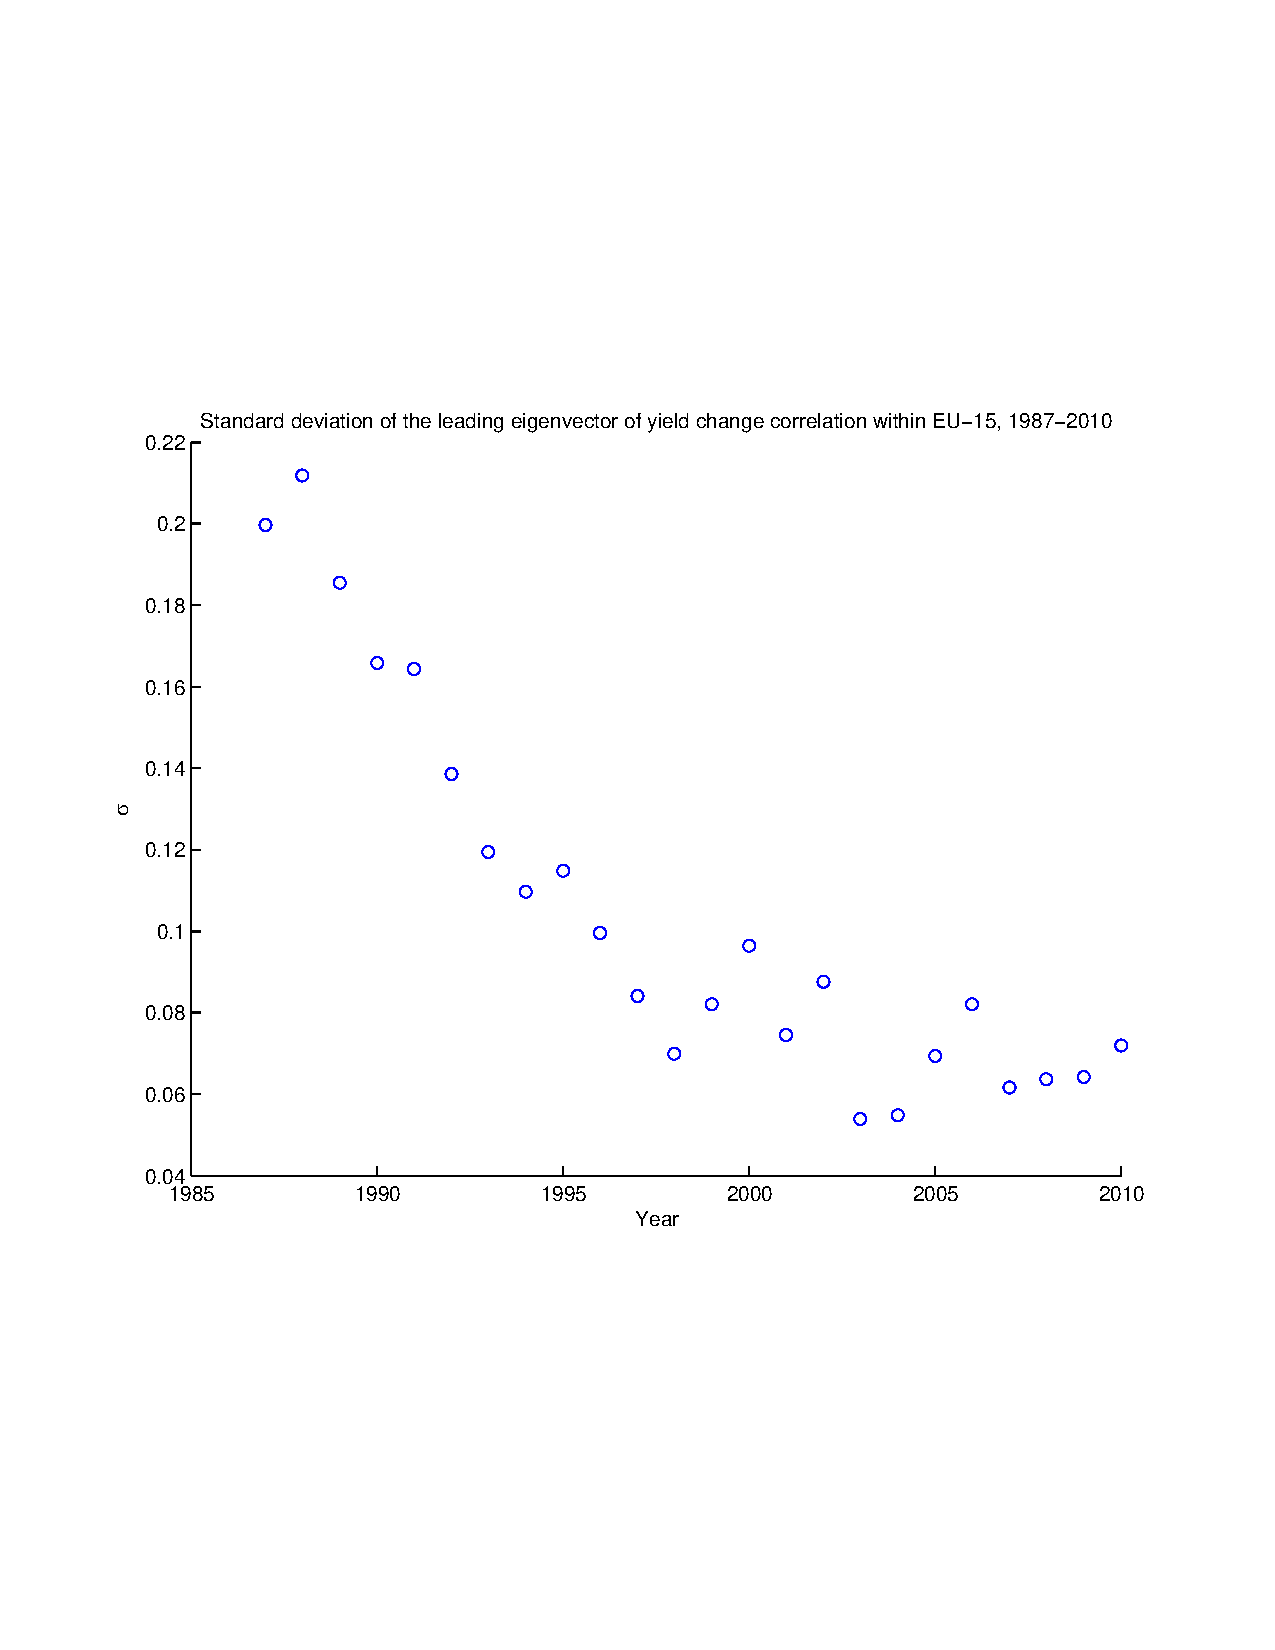
\includegraphics[width=7cm]{fig_diff_maxeigstd_eu15}
	\end{tabular}
	\caption{(a) Left, maximum eigenvalue and (b) Right, standard deviation of leading eigenvector of correlation of ten-year yields first-difference within the EU-15 member countries, 1987-2010.}
	\label{fig:diff_maxeig_eu15}
\end{figure}

\section{Discussion}
\label{sec:discussion}
In order to better understand the results presented above, I divide the 1958-2010 EU-12 sample into eight periods.  Then, I repeat the yield spread and correlation analysis above, pooling all data points within these periods.  These eight periods and the reasoning behind their choice are described below:

\begin{enumerate}
	\item 1958-1966: This period begins with the formation of the European Economic Community and ends just following the Luxembourg Compromise of 1966.
	\item 1966-1973: This period begins with the Luxembourg Compromise of 1966 and ends with the expansion of the EEC to include Denmark, Ireland, and the United Kingdom.
	\item 1974-1978: This period begins with the newly expanded EEC and ends with the proposal of the Exchange Rate Mechanism and European currency unit.
	\item 1979-1985: This period begins with the proposal of the ERM and ECU and ends just prior to the Single European Act of 1986.
	\item 1986-1992: This period begins with the Single European Act and ends just prior to the Treaty of Maastricht.
	\item 1993-1998: This period begins with the Treaty of Maastricht and ends just prior to the adoption of the Euro in 1999.
	\item 1999-2008: This period begins with the adoption of the Euro in 1999 and ends with the global crisis of late 2008.
	\item 2009-2010: This period captures the recent global and Eurozone crises.
\end{enumerate}


\begin{table}[ht!]
	\centering
	\begin{tabular}{|c|c|c|}
		\hline
		\textbf{Years} & \textbf{Mean Spread} & \textbf{Standard Deviation of Spread}\\\hline
1958-1966 & 1.107 & 0.768\\\hline
1967-1973 & 1.030 & 0.809\\\hline
1974-1978 & 4.823 & 2.912\\\hline
1979-1985 & 5.406 & 3.463\\\hline
1986-1992 & 3.156 & 2.346\\\hline
1993-1998 & 1.343 & 1.202\\\hline
1999-2008 & 0.208 & 0.186\\\hline
2009-2010 & 0.650 & 0.655\\\hline
	\end{tabular}
	\caption{Timeline from EEC to Present of Spread Measures.}
	\label{tab:timeline_spread}
\end{table}

\begin{table}[ht!]
	\centering
	\begin{tabular}{|c|c|c|}
		\hline
		\textbf{Years} & \textbf{Correlation Max. Eigenvalue} & \textbf{Difference Correlation Max. Eigenvalue}\\\hline
1958-1966 & 0.577 & 0.169\\\hline
1967-1973 & 0.675 & 0.190\\\hline
1974-1978 & 0.565 & 0.207\\\hline
1979-1985 & 0.662 & 0.151\\\hline
1986-1992 & 0.445 & 0.214\\\hline
1993-1998 & 0.956 & 0.533\\\hline
1999-2008 & 0.948 & 0.736\\\hline
2009-2010 & 0.705 & 0.465\\\hline
	\end{tabular}
	\caption{Timeline from EEC to Present of Correlation Measures.}
	\label{tab:timeline_eig}
\end{table}

Tables \ref{tab:timeline_spread} and \ref{tab:timeline_eig} present the spread and eigenvalue calculations over these periods.  The first of these periods is defined by the Luxembourg Compromise and the politics that preceded it (\cite{Garret1995}).  During the first decade of the EEC, Charles de Gaulle held the presidency of France.  de Gaulle opposed the expansion of the EEC, both in number of member states and in economic authorities.  The industry that de Gaulle was most interested in protecting was agriculture, and the negotiations over the Common Agricultural Policy therefore led to significant disagreement among France and other member states.  Following a break down in these negotiations in late June of 1965, de Gaulle removed the French representative from Brussels in protest.  This uncertainty over the future path of the economic union led to a significant increase in the absolute value of mean yield spread.  At the end of January 1965, the mean spread stood at 49.5bps, but by the end of July 1966, it had risen to nearly 201bps.  Though there is no previous period to compare the values in the tables, the eigenvalues of this period are at or very close to their minimum over the entire dataset.

The following period begins with thawing EEC member relations after the Luxembourg Compromise.  In 1969, Charles de Gaulle's presidency ended after a failed referendum, removing de Gaulle's veto and opening the door to further EEC expansion.  During this period, yield spreads improved significantly, hovering near zero even after the collapse of Bretton Woods in 1971.  In early 1973, Denmark, Ireland, and the United Kingdom enter the EEC and yields remain stable near zero in the early half of the year.  However, later in 1973, the oil crisis and US recession had begun.  Though we see an improvement in integration as measured by spread following the removal of de Gaulle and leading up to EEC expansion, the later economic turmoil leads to a significant increase in yields at the end of this period and little change in mean spreads from the previous period.  However, as measured by the correlation eigenvalues, yield comovement indicates increased integration over this period.

The following period is marked by crisis and a significant deterioration in yield spreads.  From 1974 to 1978, the mean spread over the German bund was 482bps, over four times as high as the previous two periods.  This is partially explained by Germany's strongly anti-inflationary stance as a result of Wiemar collapse and the rise of the Nazis.  The correlation analysis, however, does not paint as extreme of a picture.  The eigenvalues for yield correlation have only decreased back to 1958-1963 levels, as some of the change in yield spread is likely due to increased volatility, not actual disintegration.  Furthermore, the eigenvalues of the yield difference correlation have increased.  This is easily explained by the fact that yields are driven by exogenous events that simultaneously affect risk across states, such as the oil crisis and the US recession.  In December of 1978, the Council meets and lays out a plan for a European Exchange Rate Mechanism (ERM) and currency (ECU), the predecessor to the Euro.  Despite this plan to normalize exchange rates and currencies  in post-Bretton Woods Europe, the period from 1979 to 1985 is characterized more volatility.  The mean yield spread again increase, from 482bps in the prior period to 540bps in this period.  However, the increase of the eigenvalue of the yield correlation matrix indicates that integration is not necessarily falling during this period.  Just as in the prior period, volatility likely explains a large amount of the change in yields, not disintegration.

In 1986, member states met to sign the Single European Act.  This act was designed to set a path for a single or ``common'' market system among the member states, and, as expected, mean yield spreads continued to decline in this period.  However, the landscape of Europe underwent significant changes during this period.  First, German reunification following the fall of the Berlin Wall created uncertainty as to the economic and political landscape of Europe.  What would a unified Germany look like, and what would its political preferences be?  Would the rest of eastern Europe leave the Soviet Union, and,  if so, would they liberalize their economies and seek accession?  As a result, much of the decline in yield spreads was punctuated by uncertainty caused by events surrounding the reunification of Germany and the collapse of the Soviet Union.  Yield spreads declined to an average of 316bps over this period.  However, the maximum eigenvalue of the yield correlation hits its minimum value over the post-war period.  This is likely due to the fact that there are two nearly equally important economic trends at this time - the strong drive for European integration and the uncertainty caused by the reshaping of eastern Europe and Russia.

By 1993, much of the uncertainty surrounding these factors has been removed.  While German reunification is a slow process and the new Russian state is unstable, many of the fears of the previous period have receded.  In 1993, the Maastricht Treaty and the Single European Market also take effect.  Following this Treaty and the formation of the European Union, many European countries apply for accession or agreements with the EU.  The mean yield spread declines significantly in this period, falling from 316bps in the prior period to 134bps in this period.  Furthermore, the maximum eigenvalue of yield correlation doubles from 0.445 to 0.956.  This transition is even more clear in figures \ref{fig:maxeig_eu12} and \ref{fig:diff_maxeig_eu12}.  As measured by the yield correlation eigenvalue, Europe experiences a period of unprecedented integration.

On January 1st, 1999, many EU member states retire their domestic currencies in exchange for the Euro.  These countries begin to issue debt in this new currency, removing another source of possible discrepancy between sovereign bond yields.  In this period from 1999 to 2008, we see yield spreads decline to an average of 20bps - practically zero.  As measured by yield spreads, the EU seems to have successfully integrated European markets.  Furthermore, the eigenvalue of the yield difference correlation matrix has increased from 0.53 in the previous period to 0.736 in this period.  Nearly 95\% of the variance in yield correlation and 74\% of variance in yield difference correlation are explained by a single dimension.  

The global credit crisis of late 2008 has decreased this level of integration, however.  Yield spreads have tripled in the current period, from 20bps to 65bps.  Much of this increase can be explained by ``peripheral'' European countries, and, in particular, the PIGS - Portugal, Ireland, Greece, and Spain.  Figures \ref{fig:fig_de_spread_eu9} and \ref{fig:fig_de_spread_eu12} above indicate that there is significant separation between the bulk of yield spreads and these smaller, less mature economies.  The eigenvalue of yield correlation decreased from 0.95 in the previous period to 0.70 in the current period, and the eigenvalue of yield difference correlation decreased from 0.74 to 0.47.  These decreases can be attributed to the fact that there are now two important dimensions driving these yields - the strong degree of integration among core European economies, and the property and fiscal crises of the weaker European economies.  By these measures, European integration has returned to early Maastricht levels.

In this article, I have presented a historical context of European post-war integration through the lens of sovereign debt markets.  In addition to this important basis for comparative work and policy assessment, this article also contributes an alternative to yield spread that can better capture changes in integration in the sovereign bond market. Based on standard yield spread analysis, Europe has seen periods of comparable financial integration in the early years of the EEC.  However, based on the alternative method of this article, integration did not occur until the Single European Act of 1987 and the Maastricht Treaty of 1993.  The adoption of the Euro in 1999 brought nearly a decade of unprecedented integration and stability.  Furthermore, both methods show that the recent global real estate and European fiscal crises have significantly degraded financial integration to a level not seen since Maastricht.  In future work, I hope to (1) extend this analysis to a broader set of European states and a wider range of time, (2) incorporate a more realistic model of yields to regress out known state-specific factors such as population and the debt-to-GDP ratio, and (3) perform state-specific analysis using the components of the largest eigenvectors as a proxy to state-level integration.  


\newpage
\section*{References}
\doublespacing
\begin{thebibliography}
\expandafter\ifx\csname url\endcsname\relax
 \def\url#1{\texttt{#1}}\fi
\expandafter\ifx\csname urlprefix\endcsname\relax\def\urlprefix{URL }\fi
\bibitem{Baek2005} I.-M. Baek, A. Bandopadhyaya, C. Dhu. Determinants of market-assessed sovereign risk: Economic fundamentals or market risk appetite? \textit{Journal of International Finance and Money}, 24:533-548, 2005.
\bibitem{Baillie1996} R. Baillie. Long Memory Processes and Fractional Integration in Econometrics. \textit{Journal of Econometrics}, Vol. 73 , pp.5-59, 1996.
\bibitem{Biglaiser2007} G. Biglaiser, K. DeRouen Jr. Sovereign bond ratings and neoliberalism in Latin America. \textit{International Studies Quarterly}, Vol. 51, 2007.
\bibitem{Brada2001} J. Brada, A. Kutan. The convergence of monetary policy between candidate countries and the European Union. \textit{Economic Systems}, Vol. 25:3, pp. 215-31, 2001.
\bibitem{Burik1990} P. Burik, R. Ennis. Foreign bonds in diversified portfolios: a limited advantage. \textit{Financial Analysts Journal}, Mar.-Apr., 1990.
\bibitem{Cantor1996} R. Cantor, F. Packer. Determinants and impact of sovereign credit ratings. \textit{Federal Reserve Board of New York Economic Policy Review}, 1996.
\bibitem{Cappelen1999} A. Cappelen, J. Fagerberg, B. Verspagen. Lack of regional convergence. In: \textit{The Economic Challenge for Europe. Adapting to Innovation-Based Growth}.
\bibitem{Cappelen2003} A. Cappelen, F. Castallacci, J. Fagerberg, B. Verspagen. The impact of EU regional support on growth and convergence in the European Union. \textit{Journal of Common Market Studies}, Vol. 41:4, 2003.
\bibitem{Christiansen1997} H. Christiansen, C. Pigott. Long-term interest rates in globalised markets. OECD Working Paper, 1997.
\bibitem{Clare1995} A.D. Clare, M.  Maras, S.H. Thomas. The integration and efficiency of international bond markets. \textit{Journal of Business Finance \& Accounting}, 22, pp. 313-322, 1995.
\bibitem{Clare2000} A.D. Clare, I. Lekkos. An analysis of the relationship between national bond markets. Bank of England Working Paper, 2000.
\bibitem{Conlon2009} T. Conlon, H.J. Ruskin, M. Crane. Cross-correlation dynamics in financial time series. \textit{Physica A}, Vol. 388:5, 2009.
\bibitem{Downs1996} G. Downs, D. Rocke, P. Barsoom. Is the good news about compliance good news about cooperation? \textit{International Organization}, Vol. 50, pp. 379-406, 1996.
\bibitem{Drozdz2001} S. Drozdz, F. Grummer, F. Ruf, J. Speth.  Towards identifying the world stock market cross-correlations: DAX versus Dow-Jones.  \textit{Physica A}, Vol. 294, 2001.
\bibitem{Duran2010} A. Duran, M.J. Bommarito II.  A profitable trading and risk management strategy despite transaction costs.  \textit{Quantitative Finance}, 2010.
\bibitem{Durbin1999} E. Durbin, D. Ng. Uncovering country risk in emerging market bond prices. Board of Governors of the Federal Reserve Discussion Paper, 1999.
\bibitem{EC2006} EU integration seen through statistics. European Commission, 2006.
\bibitem{ECB2004} Measuring financial integration in the Euro area. European Central Bank, Occasional Paper Series, No. 14, 2004.
\bibitem{ECB2005} Indicators of financial integration in the Euro area. European Central Bank, Occasional Paper Series, 2005.
\bibitem{ECB2007} Financial integration in Europe. European Central Bank, Occasional Paper Series, 2007.
\bibitem{Ekinci2007} M. Ekinci, S. Kalemli-Oczan, B. Sorensen. Financial integration within EU countries: The role of institutions, confidence, and trust. NBER Working Paper, 2007.
\bibitem{FRBSF2004} Monetary and financial integration: evidence from the EMU. Federal Reserve Bank of San Francisco Working Paper, 2004.
\bibitem{FRBSF2008} M. Spiegel. Monetary and financial integration in the EMU: Push or pull? Federal Reserve Bank of San Francisco Working Paper, 2008.
\bibitem{Fagerberg1996} J. Fagerberg, B. Verspagen. Heading for divergence? Regional growth in Europe reconsidered. \textit{Journal of Common Market Studies}, Vol. 34, pp. 431-448, 1996.
\bibitem{Frost2006} C. A. Frost. Credit rating agencies in capital markets: a review of research evidence on selected criticisms of agencies.  University of North Texas,  Working Paper, 2006.
\bibitem{Garret1995} G. Garrett.  From the Luxembourg compromise to codecision: Decision making in the European Union.  \textit{Electoral Studies}, Vol. 14:3, pp. 289-308, 1995.
\bibitem{GFD2010} Global Financial Data.  \url{http://www.globalfinancialdata.com/}.  Last accessed Dec. 2010.
\bibitem{Gray2009} J. Gray. International organization as a seal of approval: European Union accession and investor risk. \textit{American Journal of Political Science}, Vol. 53:4, pp. 931-949, 2009.
\bibitem{Hardle2007} W. Hardle, L. Simar. Applied Multivariate Statistical Analysis. Second edition, Springer: New York, 2007.
\bibitem{Heimo2007} T. Heimo, J. Saramaki, J.-P. Onnela, K. Kaski. Spectral and network methods in the analysis of correlation matrices of stock returns. \textit{Physica A}, Vol. 383, 2007.
\bibitem{Hernandez2001} L. Hernandez, R. Valdes. What drives contagion: Trade, neighborhood, or financial links?. \textit{International Review of Financial Analysis}, Vol. 10, pp. 203-218, 2001.
\bibitem{Hunt2009} J. P. Hunt. Credit rating agencies and the ``wordwide credit crisis'': the limits of reputation, the insufficiency of reform, and a proposal for improvement. \textit{Columbia Business Law Review}, 2009.
\bibitem{Kaminsky2002} G. Kaminsky, C. Reinhart. Financial markets in times of stress. \textit{Journal of Development Economics}, Vol. 69, pp. 451-470, 2002.
\bibitem{Kuhner2001} C. Kuhner. Financial rating agencies: are they credible? Insights into the reporting incentives of rating agencies in times of enhanced risk. \textit{Schmalenbach Business Review}, Vol. 53, 2001.
\bibitem{Laloux1998} L. Laloux, P. Cizeau, J.-P. Bouchaud, M. Potters. Noise Dressing of Financial Correlation Matrices.  \textit{Physical Review Letters}, Vol. 83:7, 1998. 
\bibitem{Laloux2000} L. Laloux, P. Cizeau, M. Potters, J. Bouchaud.  Random matrix theory and financial correlations.  \textit{International Journal of Theoretical and Applied Finance}, Vol. 3:3, 2000.
\bibitem{Laopodis2008} N.T. Laopodis. Government bond market integration within European Union. \textit{International Research Journal of Finance and Economics}, Vol. 19, pp. 56-76, 2008.
\bibitem{Laopodis2010} N. T. Laopodis. Dynamic linkages among major sovereign bond yields.  \textit{Journal of Fixed Income}, Vol. 20:1, pp.74-87, 2010.
\bibitem{Levy1988} H. Levy, Z. Lerman. The benefits of international diversification in bonds. \textit{Financial Analysts Journal}, Sep.-Oct., 1988.
\bibitem{Markowitz1952} H. Markowitz. Portfolio Selection.  \textit{Journal of Finance}, Vol. 7:1, 1952.
\bibitem{Markowitz1959} H. Markowitz.  Portfolio selection: efficient diversification of investments. John Wiley \& Sons, 1959.
\bibitem{Mccarthy2004} J. McCarthy, R. DiSario, H. Saraoglu, H.C. Li. Tests of Long-Range Dependence in Interest Rates Using Wavelets.  \textit{Quarterly Review of Economics and Finance}, Vol. 44 pp. 180-189, 2004.
\bibitem{Molle1980} W. Molle.  Regional disparity and economic development in the European Community. Westmead: Saxon House, 1980.
\bibitem{Molle1988} W. Molle, R. Cappellin. Regional impacts of community policies in Europe. Aldershot. UK. 1988.
\bibitem{Obstfeld2003} M. Obstfeld, A. Taylor. Sovereign risk, credibility, and the gold standard: 1870-1913 versus 1925-31. \textit{The Economic Journal}, Vol. 113, pp. 241-274, 2003.
\bibitem{PenaCasas2009} R. Pe\~na-Casas, P. Pochet. Convergence and divergence of working conditions in Europe: 1990-2005. Eurofound Report, 2009.
\bibitem{Schimmelfennig2005} F. Schimmelfennig, U. Sedelmeier. The Europeanization of Central and Eastern Europe. Ithaca, NY: Cornell University Press, 2005.
\bibitem{Solnik1996} B. Solnik, C. Boucrelle, Y. Le Fur. International market correlation and volatility. \textit{Financial Analysts Journal}, Sep.-Oct., 1996.
\bibitem{Tam2008} C.S. Tam, I.W. Yu. Modeling sovereign bond yield curves of the US, Japan and Germany. \textit{International Journal of Finance and Economics}, Vol. 13, pp. 82-91, 2008.
\bibitem{Vachudova2001} M. Vachudov\'a. The leverage of international institutions on democratizing states: the European Union and Eastern Europe. RSCAS Working Paper, 2001.
\bibitem{VonStein2005} J. von Stein. Do treaties constrain or screen? Selection bias and treaty compliance. \textit{The American Political Science Review}, Vol. 99:4, pp. 611-22, 2005.
\bibitem{Westphalen2001} M. Westphalen. The determinants of sovereign bond credit spreads changes. HEC Working Paper, 2001.
\bibitem{Yang2005} J. Yang. Government bond market linkages: evidence from Europe. \textit{Applied Financial Economics}, Vol. 15, pp. 599-610, 2005.
\end{thebibliography}

\newpage
\section*{Appendix A: Figures}
\begin{figure}[h]
	\centering
	\includegraphics[width=9cm]{fig_data_eu9}
	\caption{Data availability by year for the EU-9 dataset}
	\label{fig:data_eu9}
\end{figure}

\begin{figure}[h]
	\centering
	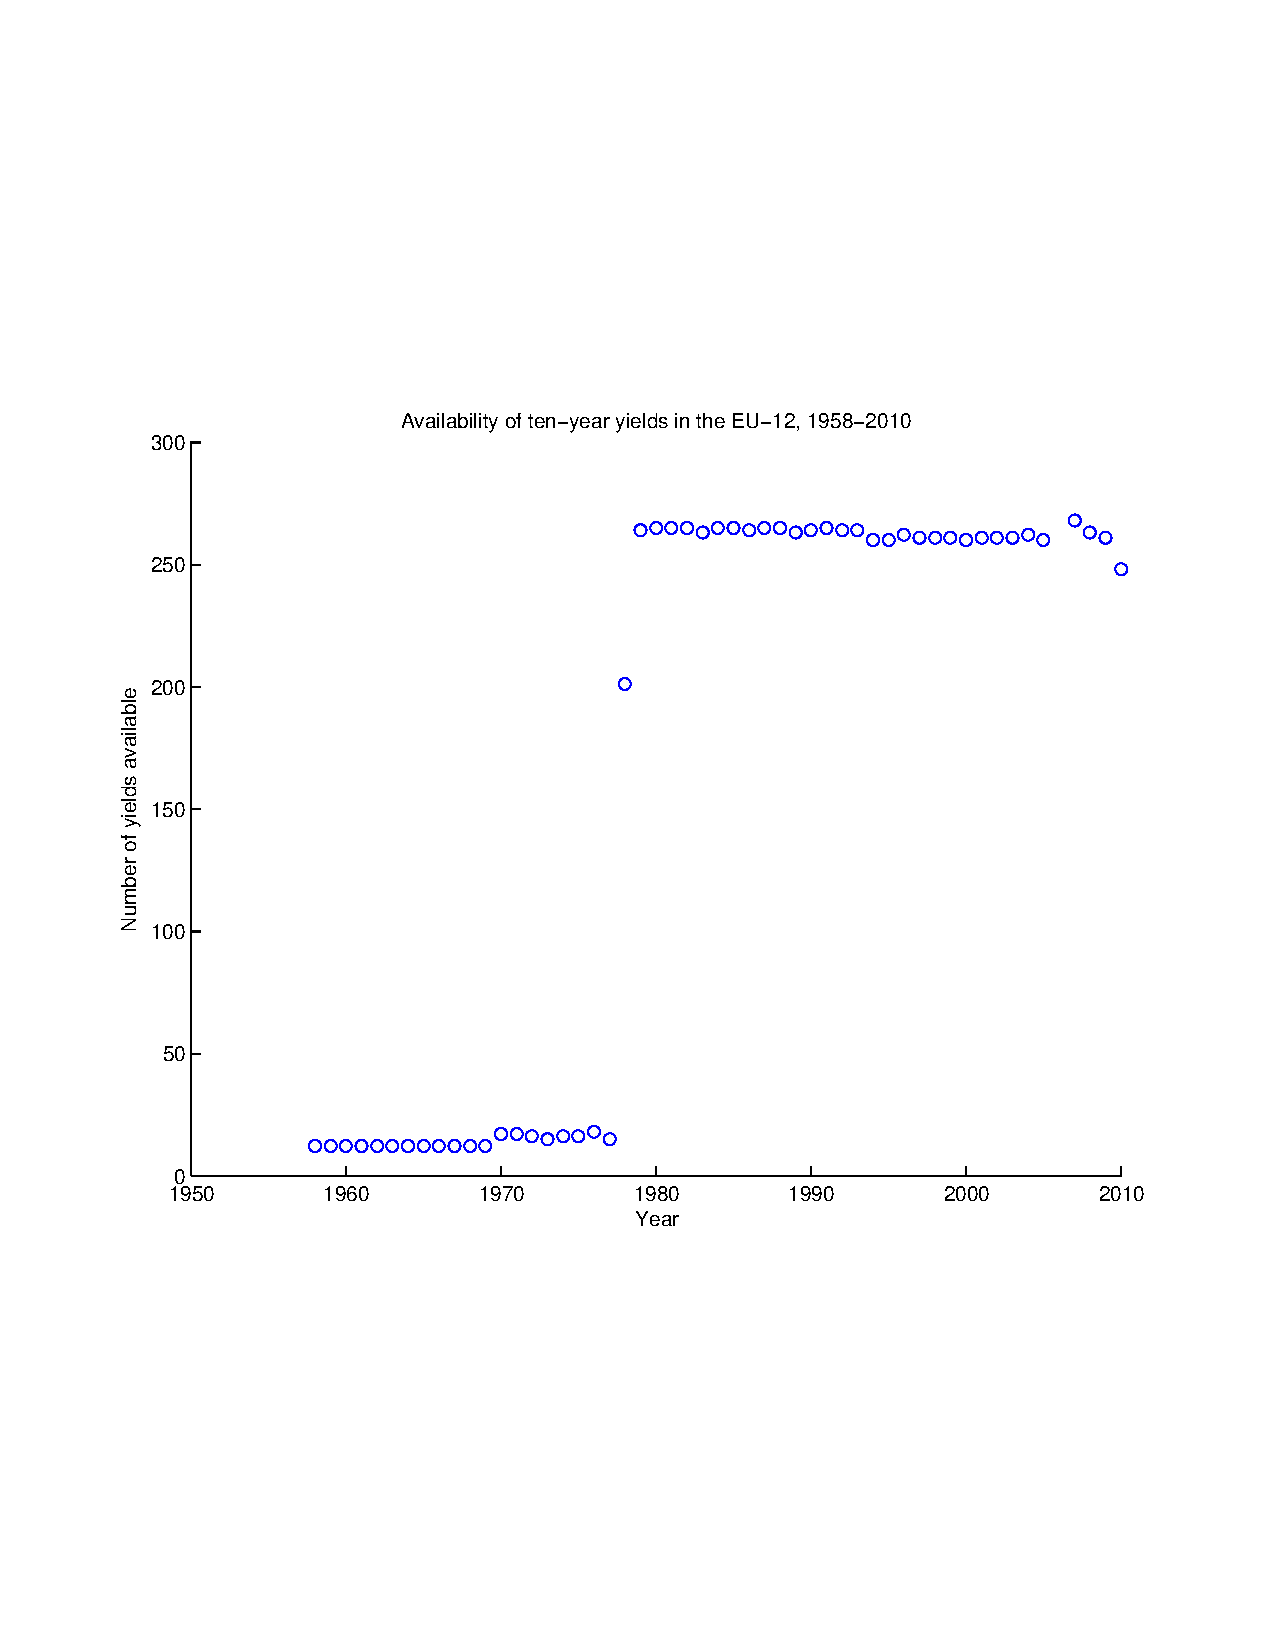
\includegraphics[width=9cm]{fig_data_eu12}
	\caption{Data availability by year for the EU-12 dataset}
	\label{fig:data_eu12}
\end{figure}

\begin{figure}[h]
	\centering
	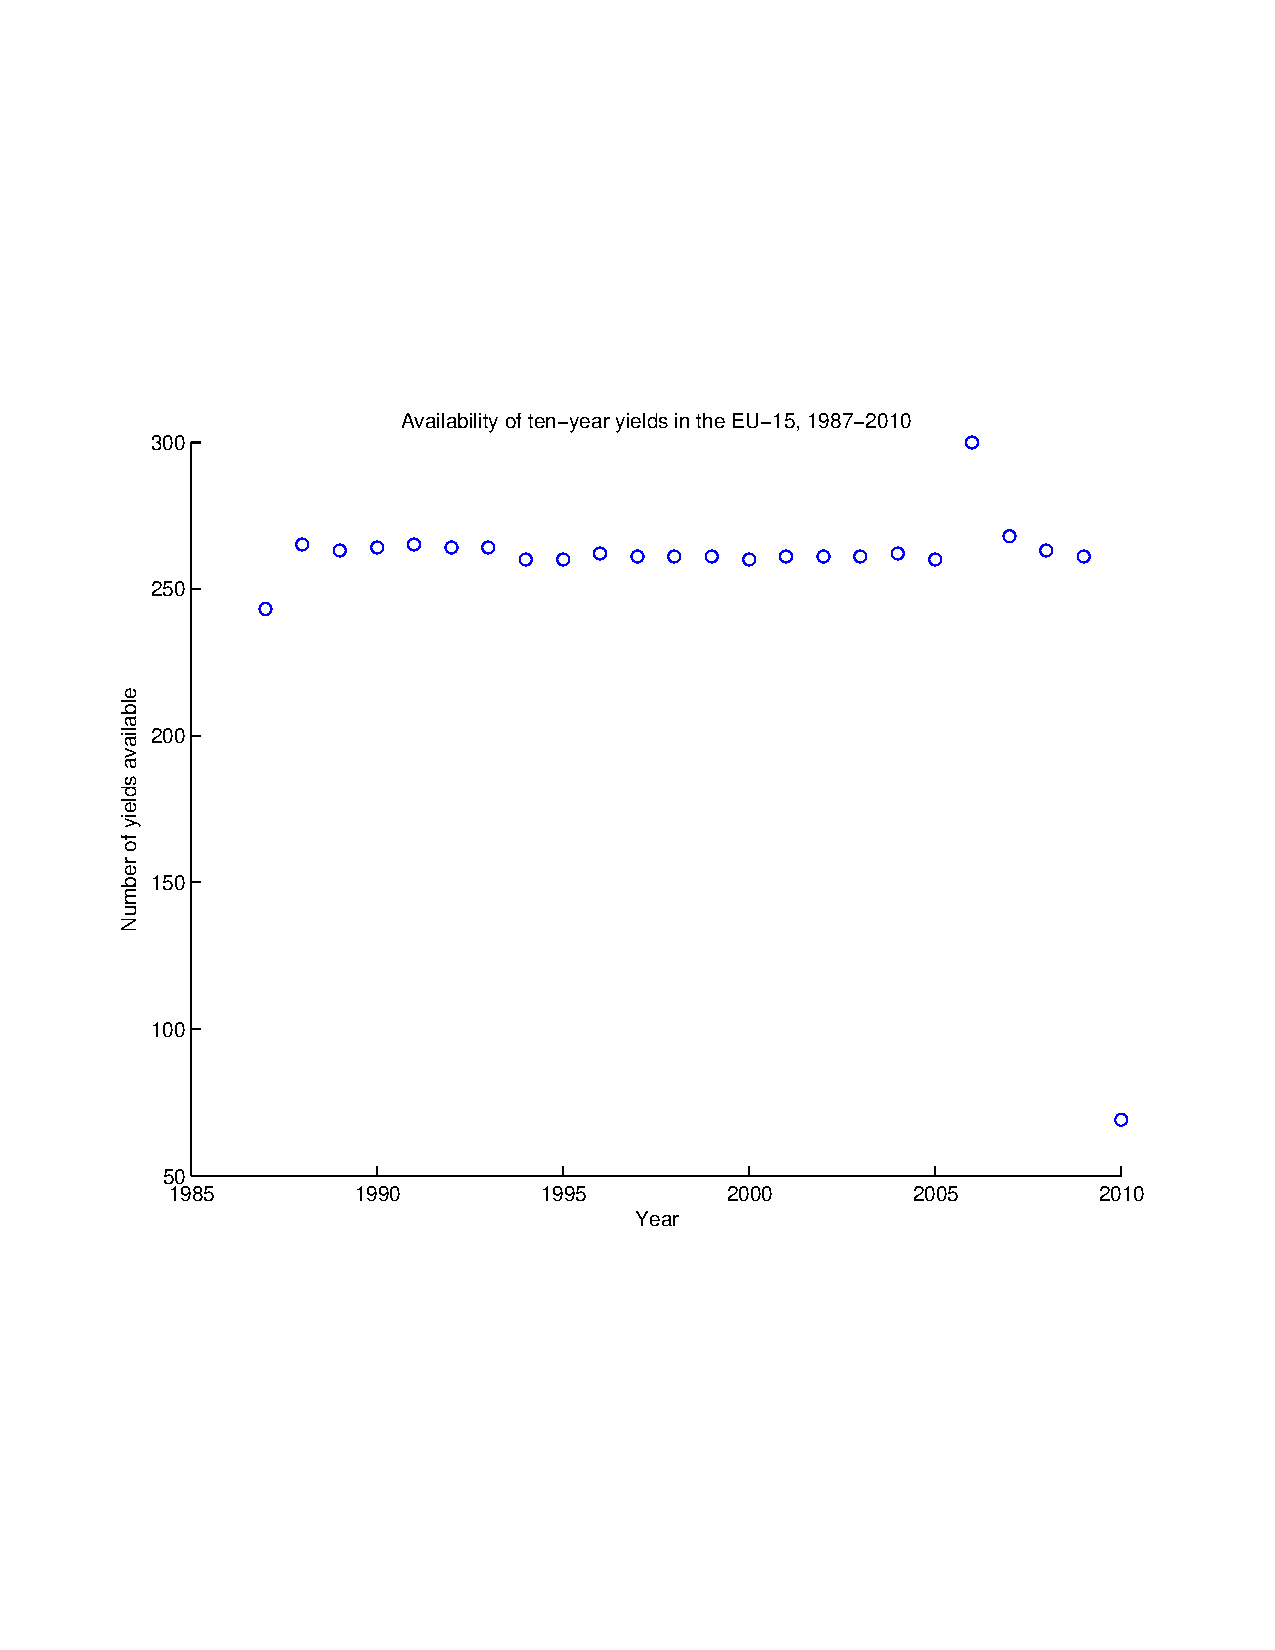
\includegraphics[width=9cm]{fig_data_eu15}
	\caption{Data availability by year for the EU-15 dataset}
	\label{fig:data_eu15}
\end{figure}
\end{document}